\documentclass[a4paper, 12pt]{article}
\usepackage{graphicx}
\usepackage[margin=1in]{geometry}
\usepackage{titlesec}
\usepackage{indentfirst}
\usepackage{setspace}
\usepackage{amsmath}
\usepackage{amssymb}
\usepackage[outputdir = ../]{minted}
\usepackage[svgnames]{xcolor}
\usepackage[hidelinks]{hyperref}
\usepackage{tabularray}
\usepackage{graphbox}
\usepackage{float}
\usepackage{comment}

\titleformat{\section}[block]{\large\bfseries}{\thesection}{0.5cm}{}
\titleformat{\subsection}[block]{\normalfont\bfseries}{\thesubsection}{0.5cm}{}
\titlespacing{\subsection}{8pt}{8pt}{8pt}

\newcommand\mefvm{%
    \textit{m}\kern-.1em%
    \raise0.5ex\hbox{\textit{e}}\kern-.1em%
    \textit{f}\kern-.2em%
    \raise-0.5ex\hbox{\textit{v}}\kern-.05em%
    \textit{m}
}
\renewcommand{\labelitemi}{-}
\renewcommand{\labelitemii}{-}

\begin{document}
\doublespacing
\begin{titlepage}
    \begin{center}
        
\includegraphics[width=0.8\textwidth]{university1.jpg}\\
        
        \textbf{ME485: Computational Fluid Dynamics \\ Using Finite Volume Method}

        \vspace{0.5cm}
        Homework 1
            
        \vspace{1.5cm}

        \textbf{Uğur Ozan Baygeldi}\\
        \textbf{Ali Kaya}\\ 
        \textbf{Onur Kakilli}\\~\\
        Group 15
        
    \end{center}
\end{titlepage}

\section{Introduction}

This report is on the first homework of the course ME485, Computational Fluid Dynamics Using Finite Volume Method. The homework requests some implementations of gradient methods to \mefvm\!.

\section{Roadmap}

When the file \verb|grad_test.py| is ran, the code eventually runs the file \verb|system.py|. As a result, to efficiently complete the given assignment, commands were implemented according to the given order in \verb|system.py|.

\begin{itemize}
    \item Implement \verb|_make_compute_fpts| at \verb|elements.py|
    \item Implement \verb|_make_delu| and \verb|_make_avgu| to \verb|GradIntInters| and \verb|GradBCInters| classes at \verb|inters.py|
    \item Implement \verb|_make_grad_gg| and \verb|_make_grad_ls| with \verb|_grad_operator| \\at \verb|elements.py|
    \item Implement \verb|compute_L2_norm| at \verb|elements.py|
\end{itemize}\par

Writing the code this way allowed for an easier understanding of the working principles of \mefvm (and prompted fewer visits to G-304 and G-157).

\section{Implementation of \texttt{\_make\_compute\_fpts} at \texttt{elements.py}}

The function \verb|_make_compute_fpts| essentially sets the center values of variables to all of the faces of an element. To achieve this 3 for loops are used iterating over all elements for all variables and all faces of the current element. Iterating over each element is handled by the backend thus in the code no there is no \verb|self.neles| but instead \verb|i_begin| and \verb|i_end| is used. \newpage 
The code is as follows:

\begin{minted}[frame=lines,framesep=2mm,baselinestretch=1.2,bgcolor=Cornsilk,fontsize=\footnotesize,linenos]{python}
    def _make_compute_fpts(self):
        nvars, nface = self.nvars, self.nface

        def _compute_fpts(i_begin, i_end, upts, fpts):
            # Copy upts to fpts
            # fpts = np.empty((self.nface, self.nvars, self.neles))
            # print(np.shape(upts))
            for idx in range(i_begin, i_end):
                for j in range(nvars):
                    for i in range(nface):
                        fpts[i, j, idx] = upts[j, idx]

        return self.be.make_loop(self.neles, _compute_fpts)
\end{minted}
\par

For easier troubleshooting comments are used depicting how \verb|fpts| is constructed. In addition, \verb|np.shape()| was used extensively to figure out the structure of arrays that are not obvious by creating a test mesh with 9 elements. If the output of the shape was \verb|(1,9)| for example, it is understood that the first argument is variable and the second was element id. This method was employed to figure out the arguments of \verb|upts|. In further code blocks for this report, these tricks will be removed to de-clutter the code.\\\par

The code loops over; the elements with the parameter \verb|idx|, variables with the parameter \verb|j|, and faces of the current element with the parameter \verb|i|. Then, for each loop, sets the appropriate index in \verb|fpts| to the element cell center value.

\section{Implementation of \texttt{\_make\_delu} and \texttt{\_make\_avgu} to \texttt{GradIntInters} and \texttt{GradBCInters} at \texttt{inters.py}} \label{deluavgu}\label{avgu}

The functions, \verb|_make_delu| and \verb|_make_avgu| are crucial for implementing the Least-Squares and Weighted Least-Squares method, and the Green-Gauss-Cell-Based method respectively. Essentially these functions, when called, subtract or average the values of the neighbor faces of neighbor elements, with special care for the boundary conditions for the functions implemented to the \verb|GradBCInters| class.\newpage

\subsection{Implementation of \texttt{\_make\_delu}} \label{delu}

For the \verb|GradIntInters| class the following code implements \verb|_make_delu|:

\begin{minted}[frame=lines,framesep=2mm,baselinestretch=1.2,bgcolor=Cornsilk,fontsize=\footnotesize,linenos]{python}
    def _make_delu(self):
        nvars = self.nvars
        lt, le, lf = self._lidx
        rt, re, rf = self._ridx

        def compute_delu(i_begin, i_end, *uf):
            for idx in range(i_begin, i_end):
                lti, lfi, lei = lt[idx], lf[idx], le[idx]
                rti, rfi, rei = rt[idx], rf[idx], re[idx]

                for jdx in range(nvars):
                    ul = uf[lti][lfi, jdx, lei]
                    ur = uf[rti][rfi, jdx, rei]

                    delu = ur - ul

                    uf[lti][lfi, jdx, lei] =  delu
                    uf[rti][rfi, jdx, rei] = -delu

        return self.be.make_loop(self.nfpts, compute_delu)
\end{minted}
\par

The code takes the information of the main element named the left element \verb|ul|, and the adjacent element named the right element \verb|ur|. Then for each variable, finds the difference of the faces and updates the interfaces. The left face gets updated to the value of $\Delta u$ while the right face gets $-\Delta u$, where $u$ stands for an arbitrary variable. The change in sign is caused by $u$ being a vector.\\\par

For the boundary conditions, the procedure is similar. The main difference is that for the boundary condition, the right element is a predefined element constructed at \verb|bcs.py|. The code at \verb|bcs.py| simply takes the boundary conditions from the \verb|.ini| file and applies according to specified type, creating a "pretend" right element for calculation purposes.\newpage \par

For the \verb|GradBCInters| class the following code implements \verb|_make_delu|:

\begin{minted}[frame=lines,framesep=2mm,baselinestretch=1.2,bgcolor=Cornsilk,fontsize=\footnotesize,linenos]{python}
    def _make_delu(self):
        nvars = self.nvars
        lt, le, lf = self._lidx
        nf = self._vec_snorm

        bc = self.bc
        array = self.be.local_array()

        def compute_delu(i_begin, i_end, *uf):
            for idx in range(i_begin, i_end):
                ur = array(nvars)
                nfi = nf[:, idx]
                lti, lfi, lei = lt[idx], lf[idx], le[idx]

                ul = uf[lti][lfi, :, lei]
                bc(ul, ur, nfi)

                delu = ur - ul

                uf[lti][lfi, :, lei] = delu

        return self.be.make_loop(self.nfpts, compute_delu)
\end{minted}
\par

Since there is no "proper" right element, setting $-\Delta u$ value to the right face is skipped. Only the left face of the intersection is updated.

\subsection{Implementation of \texttt{\_make\_avgu}} 

Similar to the \verb|_make_delu| functions, \verb|_make_avgu| employs the same method. The main difference between the two is, obviously, \verb|_make_avgu| takes the averages of the faces and assigns them to each side of the face equally. \\\par

A simple change in the operation between the two faces is enough to implement \verb|_make_avgu| for the intersection and boundary condition classes by swapping the difference operation to an averaging operation and setting the same value on both sides. \newpage \par

For the \verb|GradIntInters| class the following code implements \verb|_make_avgu|:

\begin{minted}[frame=lines,framesep=2mm,baselinestretch=1.2,bgcolor=Cornsilk,fontsize=\footnotesize,linenos]{python}
    def _make_avgu(self):
        nvars = self.nvars
        lt, le, lf = self._lidx
        rt, re, rf = self._ridx

        def compute_avgu(i_begin, i_end, *uf):
            for idx in range(i_begin, i_end):
                lti, lfi, lei = lt[idx], lf[idx], le[idx]
                rti, rfi, rei = rt[idx], rf[idx], re[idx]

                for jdx in range(nvars):
                    ul = uf[lti][lfi, jdx, lei]
                    ur = uf[rti][rfi, jdx, rei]

                    avgu = (ul+ur)/2

                    uf[lti][lfi, jdx, lei] = avgu
                    uf[rti][rfi, jdx, rei] = avgu

        return self.be.make_loop(self.nfpts, compute_avgu)
\end{minted}
\par

Similarly for the \verb|GradBCInters| class the following code implements \verb|_make_avgu|:

\begin{minted}[frame=lines,framesep=2mm,baselinestretch=1.2,bgcolor=Cornsilk,fontsize=\footnotesize,linenos]{python}
    def _make_avgu(self):
        nvars = self.nvars
        lt, le, lf = self._lidx
        nf = self._vec_snorm
        bc = self.bc
        array = self.be.local_array()

        def compute_avgu(i_begin, i_end, *uf):
            for idx in range(i_begin, i_end):
                ur = array(nvars)
                nfi = nf[:, idx]
                lti, lfi, lei = lt[idx], lf[idx], le[idx]
                ul = uf[lti][lfi, :, lei]
                bc(ul, ur, nfi)

                avgu = (ur + ul)/2

                uf[lti][lfi, :, lei] = avgu

        return self.be.make_loop(self.nfpts, compute_avgu)
\end{minted}
\par
\subsection{Possible Problems of the Method} \label{probavgudelu}
The method assumes that the element has one boundary face. For rectangular grids with quad meshes, it is possible to encounter elements with more than one boundary face, for cases like those, a better implementation could be prepared.
\section{Implementation of \texttt{\_make\_grad\_gg} and \texttt{\_make\_grad\_ls} with \\ \texttt{\_grad\_operator} at \texttt{elements.py}}
\subsection{The Green-Gauss Cell Based Method}
The Green-Gauss method is a numerical tool used in computational fluid dynamics (CFD) to compute the gradient. This gradient can be of the type of properties such as the temperature, pressure, or velocity components at the control volume. It can be implemented on centers or nodes based on the method used to obtain the gradient. Green-Gauss is based on the divergence theorem which converts a vector field through a closed surface to a divergence of the field within the volume encapsulated by that surface. In the Green-Gauss approach, the gradient of a scalar field at the centroid of a control volume is approximated by integrating over the control volume's faces. The method assumes that the variation of the scalar field is linear within the control volume, and this is the reason why it is fast and straightforward to implement. In practice, the Green-Gauss method computes gradients by summing contributions from all the faces of a control volume. For each face, the scalar field values at the neighboring cell centers are used to calculate the value of the field at the face centroid, often interpolated linearly. 
\\\par
Normally the flux through each face is then weighted by the face's area and its normal vector, however, the scope of this homework is not to make the weighted Green Gauss method. Then the resulting gradients must be divided by volume to maintain conservation properties and accuracy. 
\subsection{Mathematical Implementation of the Green-Gauss Cell Based Method}
By utilizing the Divergence Theorem, one can convert the volume integral to surface integral as shown below.

\begin{equation}
    \int_{V}^{}{(\nabla\cdot\phi)dV} = \oint_{S}^{}{(\phi\cdot n) dS}
\end{equation}

Then one may utilize the above equality to find the gradient as given below, where \(\nabla\phi_{e}\) is gradient at the center of the element, \(V_{e}\) is the volume of the respective element, \(\phi_{f}\) is the face values, \(n_{f}\) is the unit normal of the face, \(N_{f}\) is the number of faces and \(S_{f}\) is the surface area of the respective element's respective face.

\begin{equation}
    \nabla\phi_{e} = \frac{1}{V_{e}}\sum_{i = 1}^{N_{f}}{\left( \phi_{f}n_{f} \right)S_{f}}
\end{equation}

\subsection{Implementation of \texttt{\_make\_grad\_gg}}

When \verb|system.py| is observed, it can be seen that before calling \verb|_make_grad_gg|, \mefvm calls \verb|compute_avgu| for boundary and element interfaces. From \hyperref[avgu]{\textit{section 4}} of this report, recall that \verb|compute_avgu| which calls \verb|_make_avgu| adjusts the flux point array, \verb|fpts|, such that every side of every element has the value of neighbor faces values averaged. \\\par

To calculate the gradient, the code loops over every element, for every element another loop, loops over every dimension, for every dimension another loop, loops over every variable, and lastly for every variable another loop loops over every face of the element. For every variable, a sum is calculated by adding up all the values of faces. The sum is then simply placed at the appropriate spot in the \verb|grad| array. To be used later on while calculating the error or when necessary for further assignments.\newpage\par

The following code implements \verb|_make_grad_gg|

\begin{minted}[frame=lines,framesep=2mm,baselinestretch=1.2,bgcolor=Cornsilk,fontsize=\footnotesize,linenos]{python}
    def _make_grad_gg(self):

        nface, ndims, nvars = self.nface, self.ndims, self.nvars
        # Normal vector and volume
        snorm_mag = self._mag_snorm_fpts # face | elemid
        snorm_vec = np.rollaxis(self._vec_snorm_fpts, 2) # x,y | face | elemid
        vol       = self._vol # elemid
        def _cal_grad(i_begin, i_end, fpts, grad):
            # Elementwise loop starts here
            for idx in range(i_begin, i_end):
                for d in range(ndims):
                    for j in range(nvars): # = 1
                        sum = 0
                        for i in range(nface):
                            sum += fpts[i,j,idx]*snorm_mag[i,idx]*snorm_vec[d,i,idx]

                        grad[d,j,idx] = (1/vol[idx])*sum

        return self.be.make_loop(self.neles, _cal_grad)
\end{minted}
\par
\subsection{Comments for the Green-Gauss Cell Based Method}
While the Green-Gauss method is widely used due to its simplicity, its accuracy can be affected in cases where the mesh is highly distorted which will be inspected in detail with different mesh resolutions and types. Furthermore, if the scalar field varies significantly, the accuracy of this method drops severely. Furthermore, the limitations previously mentioned on \hyperref[probavgudelu]{\textit{section 4.3}} also applies as the method calls \verb|_make_avgu| at the boundaries.

\subsection{The Least Squares Gradient Method}
The least squares method is another technique used in CFD solvers for calculating gradients. Unlike the Green-Gauss method, which was explained previously, the least squares method directly minimizes the error between the computed gradients and the differences in field values between neighboring cells. This approach works better than Green Gauss in both structured and unstructured meshes. Thus, making it more suitable for complex geometries that require complex mesh structures. The method creates a system of equations using the field values at neighboring nodes or cell centers, and it constructs an over-determined system with more linearly independent equations than unknown quantities.
\\\par
In practice, the least squares gradient evaluation starts by selecting a set of neighboring cells for a given control volume. For each neighbor, the solver calculates the difference in the scalar or vector field value and divides it by the vector distance between the cell centers. These differences are used to construct a system of equations representing the gradient components. 
\subsection{Mathematical Implementation of the Least Squares Method} \label{matlsq}
One can calculate the gradient of elements at the center by using the
following equation:
\begin{equation}
    \phi_{e_{i}} = \phi_{e_{0}} + {(\nabla\phi)_{e}}_{0}({r_{e}}_{i} - {r_{e}}_{0})
\end{equation} \par
But when using this approach, there will be three different gradient
values for the same center point. Since this is physically impossible,
one needs to choose the best available one. To do so the following
equation where n is the number of elements may be utilized.

\begin{equation}
    A = \begin{bmatrix}
x_{1} - x_{0} & y_{1} - y_{2} \\
x_{2} - x_{0} & y_{2} - y_{0} \\
\begin{matrix}
 \vdots \\
x_{n} - x_{0} \\
\end{matrix} & \begin{matrix}
 \vdots \\
y_{n} - y_{0} \\
\end{matrix} \\
\end{bmatrix}\ \ \ \ \ x = \begin{bmatrix}
\dfrac{\partial\phi}{\partial x} \\[6pt]
\dfrac{\partial\phi}{\partial x} \\
\end{bmatrix}_{e_{0}}\ \ b = \begin{bmatrix}
{\phi_{e}}_{1} - {\phi_{e}}_{0} \\
\phi_{e_{2}} - {\phi_{e}}_{0} \\
\begin{matrix}
 \vdots \\
\phi_{e_{n}} - \phi_{e_{0}} \\
\end{matrix} \\
\end{bmatrix}
\end{equation}

\begin{equation}
    Ax = b
\end{equation}

Since matrix A is not square matrix, multiplying both sides with
\(A^{T}\) is not an option. Instead, one may use pseudo inverse method.

\begin{equation}
    x = \left( A^{T}A \right)^{- 1}A^{T}b
\end{equation}

\subsection{Implementation of \texttt{\_make\_grad\_ls} with \texttt{\_grad\_operator}}
To begin with the implementation of the Least Squares Gradient method, as the code requires the operator, \verb|op|, as an input, one must first implement \verb|_grad_operator|. Thankfully, the \verb|_grad_operator| code could be sourced from the \verb|base\elements.py| file, as an added bonus, this operator also includes weight options and a hybrid method. Essentially \verb|_grad_operator| creates the $A$ matrix and then takes the inverse of it using the least squares method. \\\par
The code for \verb|_grad_operator| (with proper citation) is as follows:
\begin{minted}[frame=lines,framesep=2mm,baselinestretch=1.2,bgcolor=Cornsilk,fontsize=\footnotesize,linenos]{python}
    def _grad_operator(self):
        # Difference of displacement vector (cell to cell)
        # (Nfaces, Nelements, dim) -> (dim, Nfaces, Nelements)
        dxc = np.rollaxis(self.dxc, 2)
        # (Nfaces, Nelements)
        distance = np.linalg.norm(dxc, axis=0)

        # Code taken directly from base\elements.py, thanks hocam :)

        # Normal vector and volume
        snorm_mag = self._mag_snorm_fpts
        snorm_vec = np.rollaxis(self._vec_snorm_fpts, 2)
        vol = self._vol

        if self._grad_method == 'least-square':
            beta, w = 1.0, 1.0
        elif self._grad_method == 'weighted-least-square':
            # Invserse distance weight
            beta, w = 1.0, 1 / distance ** 2
        elif self._grad_method == 'green-gauss':
            beta, w = 0.0, 1.0
        elif self._grad_method == 'hybrid':
            # Shima et al., Green–Gauss/Weighted-Least-Squares
            # Hybrid Gradient Reconstruction for
            # Arbitrary Polyhedra Unstructured Grids, AIAA J., 2013
            # WLSQ(G)
            dxf = self.dxf.swapaxes(0, 1)

            dxcn = np.einsum('ijk,ijk->jk', dxc, snorm_vec)
            dxfn = np.einsum('ijk,ijk->jk', dxf, snorm_vec)

            w = (2 * dxfn / dxcn) ** 2 * snorm_mag / distance

            # Compute blending function (GLSQ)
            ar = 2 * np.linalg.norm(self.dxf, axis=1).max(
                axis=0)*snorm_mag.max(axis=0) / vol
            beta = np.minimum(1, 2 / ar)
        else:
            raise ValueError("Invalid gradient method : ", self._grad_method)

        # Scaled dxc vector
        dxcs = dxc * np.sqrt(w)

        # Least square matrix [dx*dy] and its inverse
        lsq = np.array([[np.einsum('ij,ij->j', x, y)
                         for y in dxcs] for x in dxcs])

        # Hybrid type of Ax=b
        A = beta * lsq + 2 * (1 - beta) * vol * np.eye(self.ndims)[:, :, None]
        b = beta * dxc * w + 2 * (1 - beta) * 0.5 * snorm_vec * snorm_mag

        # Solve Ax=b
        op = np.linalg.solve(np.rollaxis(
            A, axis=2), np.rollaxis(b, axis=2)).transpose(1, 2, 0)

        return op
\end{minted}
\par
The grad operator, as explained previously in \hyperref[matlsq]{\textit{section 5.6}} is simply the inverse of the matrix $A$ in the equation $Ab=x$. With $(A^T\!A)^{-1}A^T$ known, it is easy to compute the gradient if $b$ is known. Tracing the steps in \verb|system.py| it is found that \verb|_make_delu| is called which recalling from \hyperref[avgu]{\textit{section 4}} updates \verb|fpts| with the difference of faces, essentially converting \verb|fpts| to the matrix $b$. Then, similar to the Green-Gauss Cell Based Method, the gradient is calculated by means of nested for loops iterating over the elements, dimensions, variables, and faces. Multiplying the appropriate element of the \verb|op|, which is the grad operator, with the appropriate element of \verb|fpts|. Summing the results for every face of the element, as the values obtained are vectoral with respect to the dimension, then placing the sum to the appropriate location in \verb|grad| to obtain the gradient.\newpage\par
The following code implements \verb|_make_grad_ls|:
\begin{minted}[frame=lines,framesep=2mm,baselinestretch=1.2,bgcolor=Cornsilk,fontsize=\footnotesize,linenos]{python}
    def _make_grad_ls(self):
        nface, ndims, nvars = self.nface, self.ndims, self.nvars
        # Gradient operator 
        op = self._grad_operator
        def _cal_grad(i_begin, i_end, fpts, grad):
            # Elementwiseloop
            for idx in range(i_begin, i_end):
                for d in range(ndims):
                    for j in range(nvars):  # = 1
                        sum = 0
                        for i in range(nface):
                            sum += fpts[i, j, idx] * op[d, i, idx]

                        grad[d, j, idx] = sum

        # Compile the function
        return self.be.make_loop(self.neles, _cal_grad)    
\end{minted}
\subsection{Comments for the Least Squares Gradient Method}
\par
Solvers typically apply a weighting scheme based on the distance or cell connectivity to account for mesh irregularities, on the other hand, our solver didn’t do this for now. This will create accuracy problems while calculating gradient which will be discussed with different examples later. \\\par Once the system is solved, the resulting gradient at the cell center is still more accurate than Green-Gauss in distorted or skewed meshes. However, this method is computationally more included due to the more steps of linear operators like matrix inversion or factorization. Still, its robustness and improved accuracy for non-uniform meshes make it a preferred choice in modern CFD.

\section{Implementation of \texttt{compute\_L2\_norm} at \texttt{elements.py}}
The $L_2$ error norm is used widely in the world of CFD to determine how accurate the solver is.
\subsection{Mathematical Implementation of the $L_2$ error norm}
Assume \(X\) is an \(Nx\textit{2}\) matrix, such that all x and y coordinates of
all elements are stored in it. Where $N$ is the number of elements.

\begin{equation}
\begin{matrix}
X = \begin{bmatrix}
\begin{matrix}
x_{1} \\
x_{2} \\
x_{3} \\
\vdots \\
x_n
\end{matrix} & \begin{matrix}
y_{1} \\
y_{2} \\
y_{3} \\
\vdots \\
y_n
\end{matrix} \\
\end{bmatrix} \\
\end{matrix}
\end{equation}

To calculate the \(L_{2}\) error norm, first one needs to calculate the exact gradient. To do so one may utilize the following equations for the given test gradient. Where subscript $i$ shows \(i^{th}\) element.
\begin{equation}
\begin{matrix}
\nabla_{exact_{i}} = \begin{bmatrix}
\dfrac{x_{i}}{\sqrt{x_{i}^{2} + y_{i}^{2}}} & \dfrac{y_{i}}{\sqrt{x_{i}^{2} + y_{i}^{2}}} \\
\end{bmatrix}\  \\
\end{matrix}
\end{equation}

After calculating \(\nabla_{exact}\) at the cell center, the error can be calculated by expanding the result into the whole cell volume by multiplying with the element volume. Now one can calculate the \(L_{2}\) error norm.

\begin{equation}
\begin{matrix}
L_{2} = \sqrt{\left\lbrack \displaystyle\sum_{i = 1}^{n}\left( \nabla_{computed_{i}} - \nabla_{exact_{i}} \right)V_{i} \right\rbrack^{2}\ } \\
\end{matrix}
\end{equation}
\subsection{Implementation of \texttt{compute\_L2\_norm}}
To implement the $L_2$ error norm as mentioned in the previous subsection, one must first obtain the exact values. These exact values require the exact gradient which sadly cannot be calculated numerically and unless a symbolic differentiator is used has to be hard coded into the code. To make the implementation seamless and allow for higher dimensions, an array is used. The code once again loops through every element for every variable and dimension recording the cell center values. Then with the hard coded gradient creates the exact gradient matrix. After exact gradient is obtained, the error matrix is then formed by subtracting the exact gradient from the found gradient and multiplying the result with the element volume. Lastly to obtain the $L_2$ error norm, the $L_2$ norm of the error matrix is obtained through \verb|np.linalg.norm(err, axis=2)|.\\\par
The code for \verb|compute_L2_norm| is as follows:
\begin{minted}[frame=lines,framesep=2mm,baselinestretch=1.2,bgcolor=Cornsilk,fontsize=\footnotesize,linenos]{python}
    def compute_L2_norm(self):
        # adjust faces to eles
        nvars, neles, ndims = self.nvars, self.neles, self.ndims
        vol                 = self._vol
        xcs                 = self.xc # Cell center point (x,y)
        exactGrad = np.zeros((self.ndims, self.nvars, self.neles))
        err = np.zeros((self.ndims, self.nvars, self.neles))
        for idx in range(neles):
            x = np.zeros(ndims)
            for i in range(nvars):
                for j in range(ndims):
                    x[j] = xcs[idx][j]
                eqn = [x[0]/math.sqrt(x[0]*x[0]+x[1]*x[1]), x[1]/math.sqrt(
                    x[0]*x[0] + x[1]*x[1])] # sqrt(x^2 + y^2)
                #eqn = [2*x[0],2*x[1]] # x^2 + y^2
                #eqn = [32*(x[0]**31), 32*(x[1]]**31) # x^32 + y^32
                #eqn = [-math.sin(x[0]**2+x[1]**2)*2*x[0],
                #       -math.sin(x[0]**2+x[1]**2)*2*x[1]]
                for j in range(ndims):
                    exactGrad[j, i, idx] = eqn[j]
                    err[j, i, idx] = (self.grad[j, i, idx] - exactGrad[j, i, idx]
                                       )*vol[idx]

        resid = np.linalg.norm(err, axis=2)
        return resid
\end{minted}
\section{Tests and Results}
\subsection{Input Meshes}
The first test mesh is the mesh provided with the assignment, it is a mixed mesh with triangle and quadrilateral meshes. This mesh is easy to understand and provides a basic understanding of the \verb|gmsh| structure. To ease the test-case generation, further meshes were created with the same boundary locations as the \verb|q| value changes at the boundaries. Also considering that the report covers different equations for \verb|q| setting the boundary locations the same eliminates unnecessary calculations.\\\par
\begin{figure}[H]
    \centering
    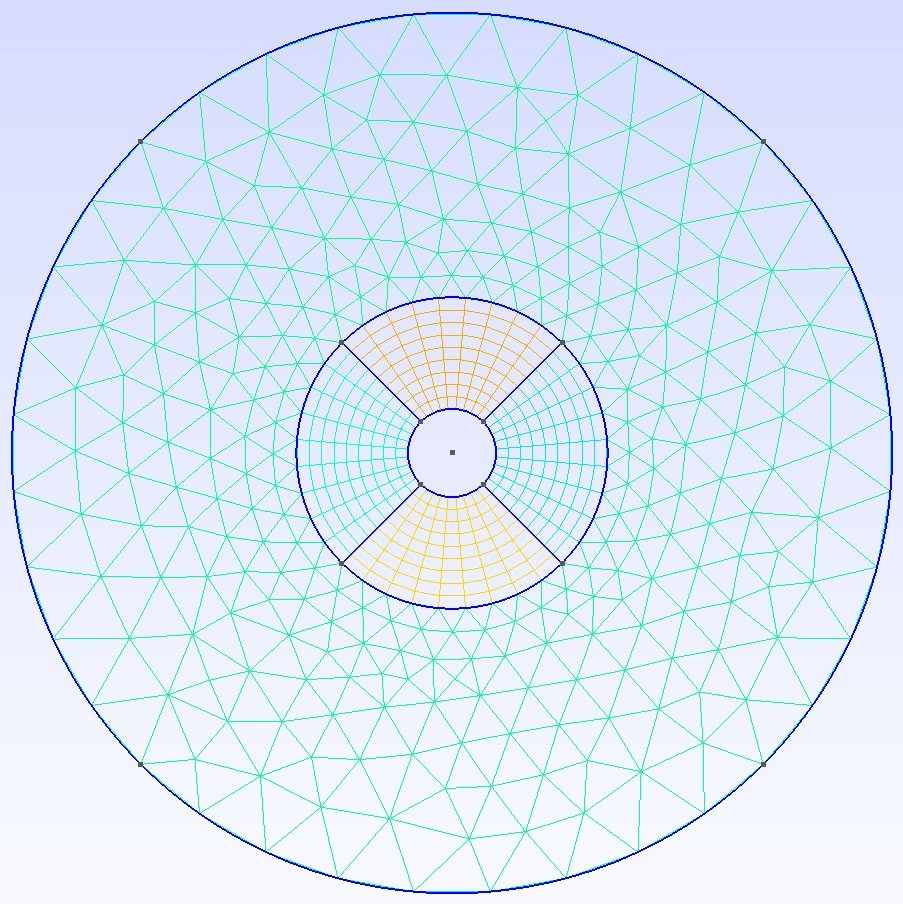
\includegraphics[width=0.3\linewidth]{grad.jpg}
    \caption{Provided Mesh (grad.msh)}
\end{figure}\par
Next mesh used is similar to the first one however uses only quadrilateral meshes. This example uses 100 uniformly placed nodes along the edges. The Python file that generates this mesh has an option to change the amount of uniformly placed nodes and this mesh will be used later on for comments as one would expect the $L_2$ error norm to get smaller with finer mesh.\\\par \label{here}
\begin{figure}[H]
    \centering
    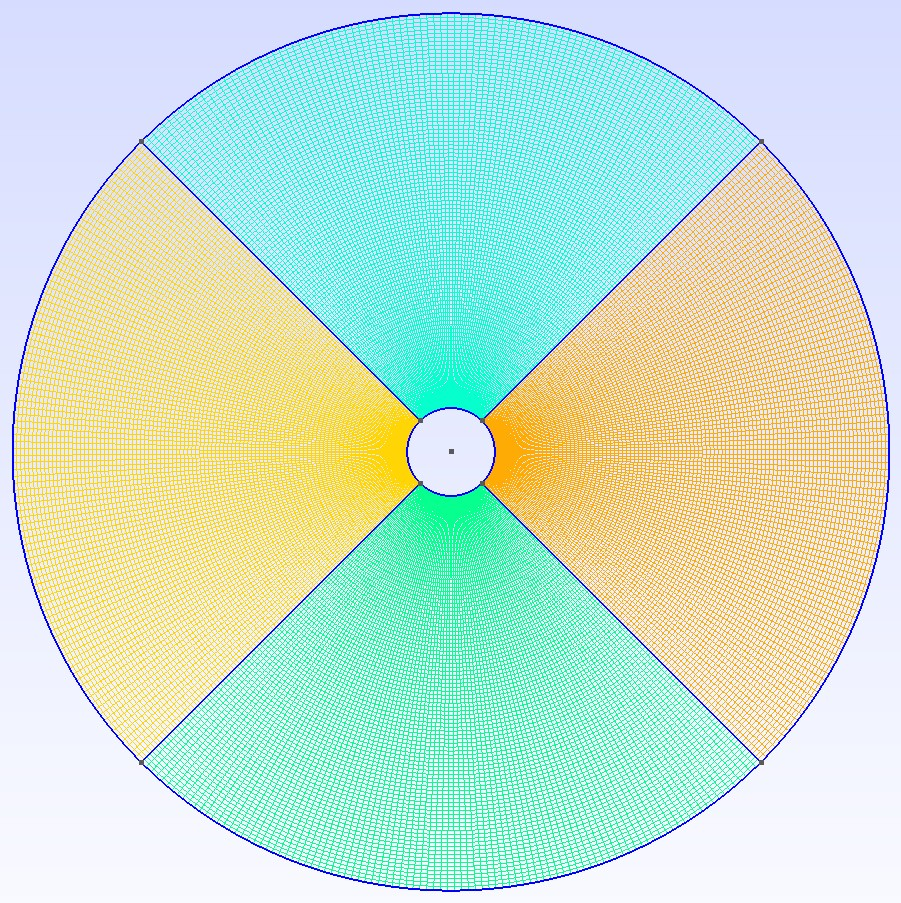
\includegraphics[width=0.3\linewidth]{grads.jpg}
    \caption{Finer Quad Mesh (grads.msh)}
\end{figure}
 Continuing with different mesh structures, the next mesh uses mixed mesh element generation method. This particular mesh is constructed to check whether the implemented gradient calculation methods work on nonconventional meshes using geometry. It consists of a circle for the inner boundary, two triangle-like regions, eight triangles, two trapezoidal, and four regions between the outer circle and the concave octagon inside. Moreover, the first two triangle-like geometries and the last region mentioned are constructed by triangle elements with no transfinite function implemented. Other regions consist of quadrilateral mesh types. \\\par
%(higher order tetra ok quad anansın amı)
\par
\begin{figure}[H]
    \centering
    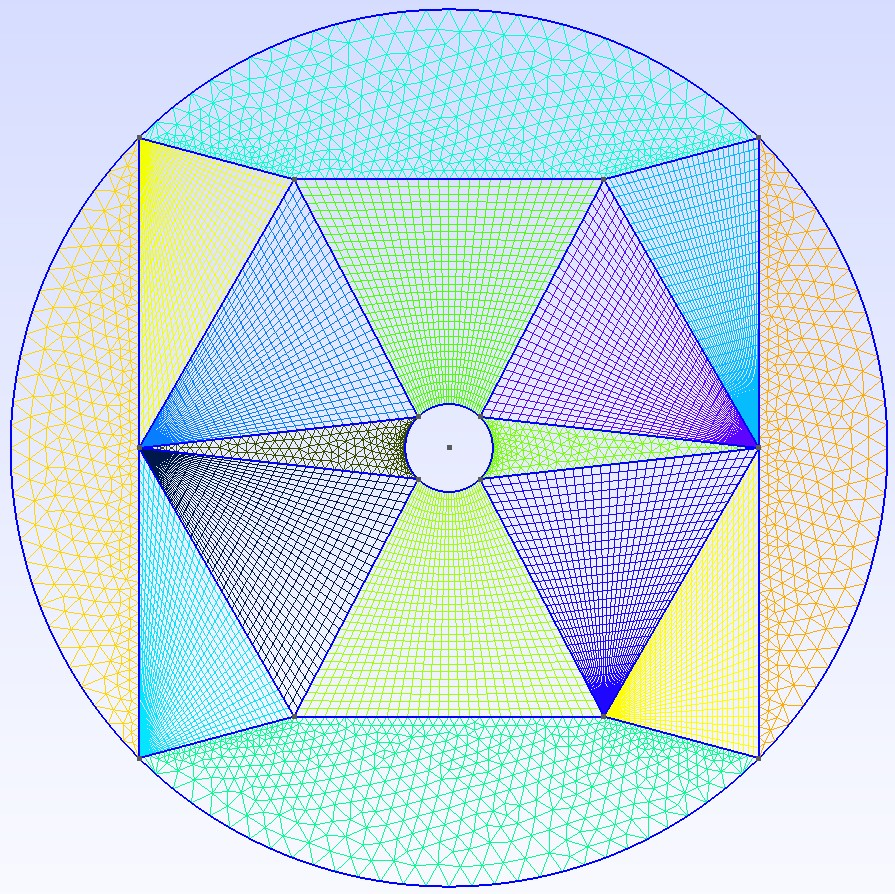
\includegraphics[width=0.3\linewidth]{onurk1.jpg}
    \caption{Weird Mesh 1 (gradok1.msh)}
\end{figure}
This particular mesh consists of highly structured rectangular mesh elements. It consists of eight subsections to create these tightly packed elements. North, east south, and west sections are divided to 9x10 and others are 10x10. This mesh is constructed to see whether structured meshes will result in lower $L_2$ norms for different cases. \\\par
\label{f4}
\begin{figure}[H]
    \centering
    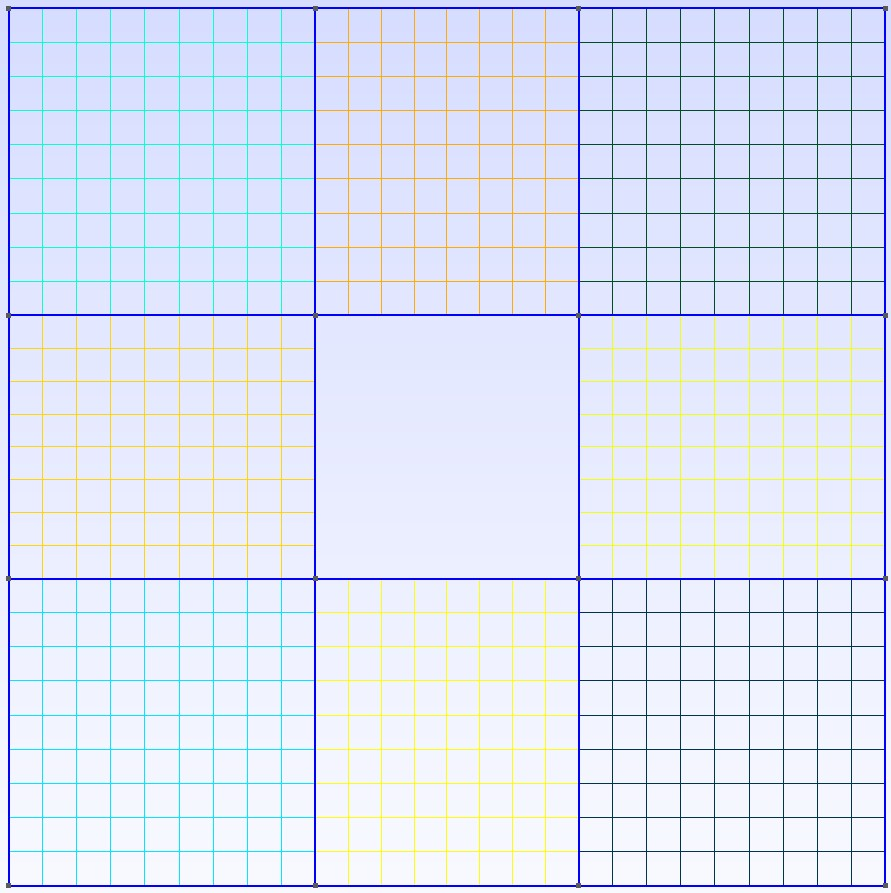
\includegraphics[width=0.3\linewidth]{onurk2.jpg}
    \caption{Box in Box Structured (gradok2.msh)}
\end{figure}
The very next mesh is similar to the previous one, it consists of two squares one inside the other and with mixed elements. Yet, this time rather than being structured, it is unstructured, and in two ways, north and south, it consists of triangular elements while the other two are quadrilateral.  \par
\begin{figure}[H]
    \centering
    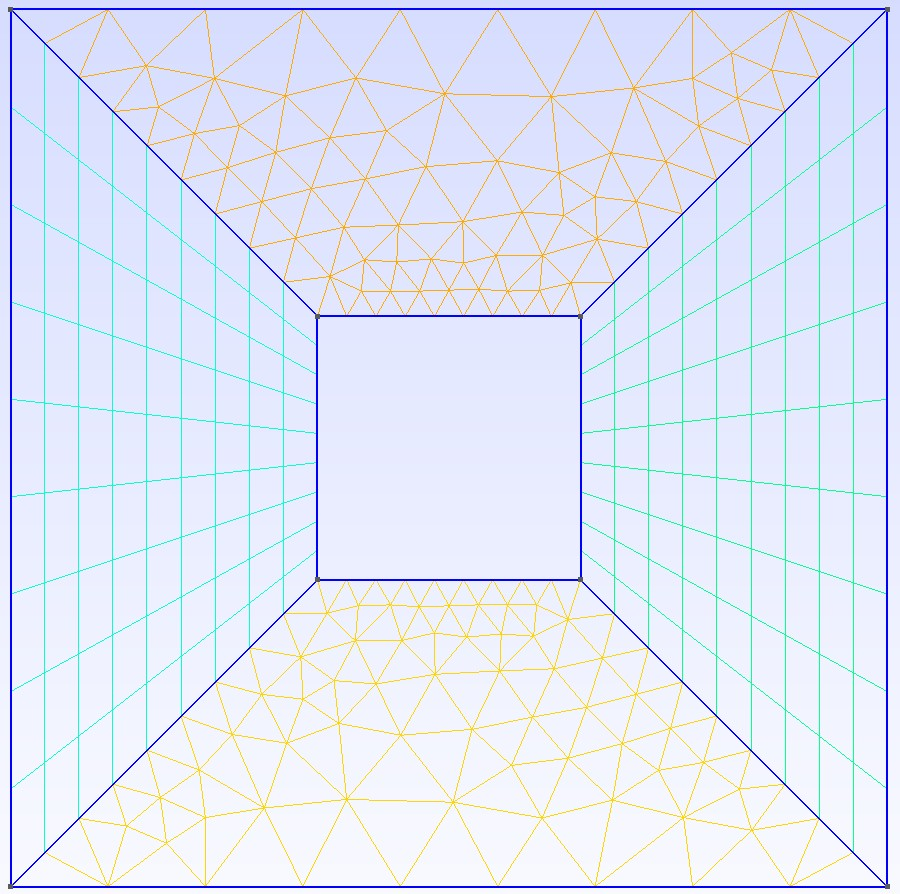
\includegraphics[width=0.3\linewidth]{onurk3.jpg}
    \caption{Box in Box Unstructured (gradok3.msh)}
\end{figure}
This mesh and the one after it were constructed with unusual geometries. The reason why is to see the effect of distorted geometries on the $L_2$ norm. Also, the orthogonality of elements is another source of error while calculating the gradient. One can see both meshes below. The first one which is called "Pointy Star in Box" consists of a concave octagon for the inner boundary, a circle to construct transfinite curves, and a square for the outer boundary.\\\par
\label{f6}
\begin{figure}[H]
    \centering
    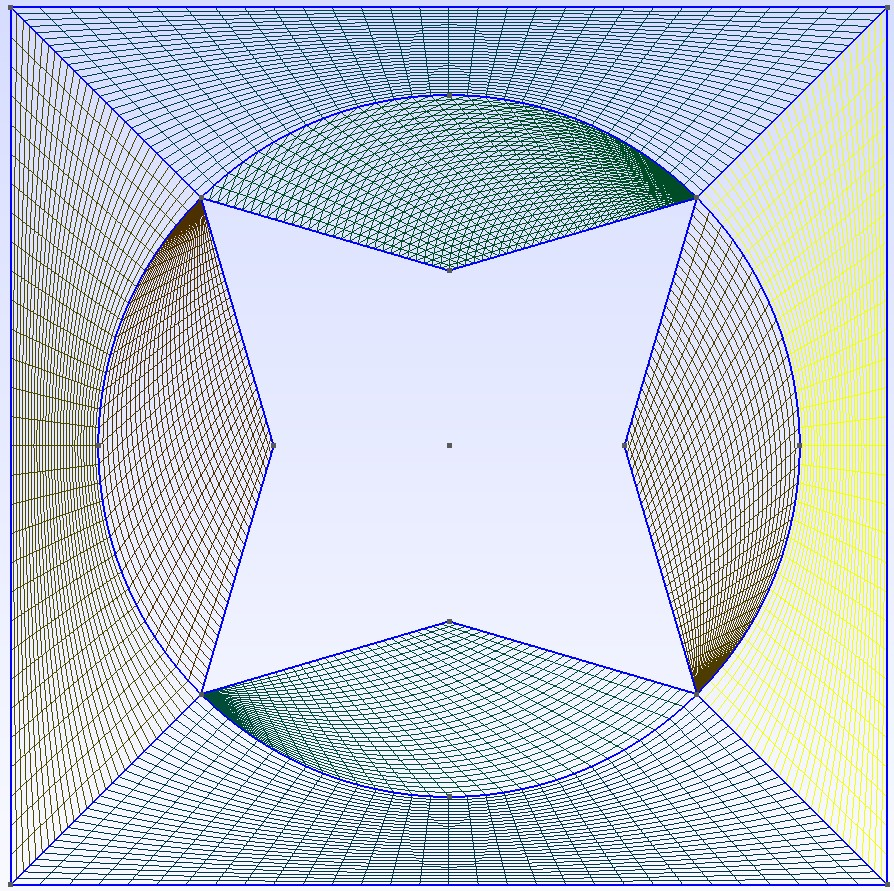
\includegraphics[width=0.3\linewidth]{alikmesh1.jpg}
    \caption{Pointy Star in Box (gradak1.msh)}
\end{figure} \par
The other mesh is called "The Eye in Box" and consists of four circle arcs with different radii and center points, a full circle centered at the origin, and lastly the outer square for the outer boundary.
\label{f7}
\begin{figure}[H]
    \centering
    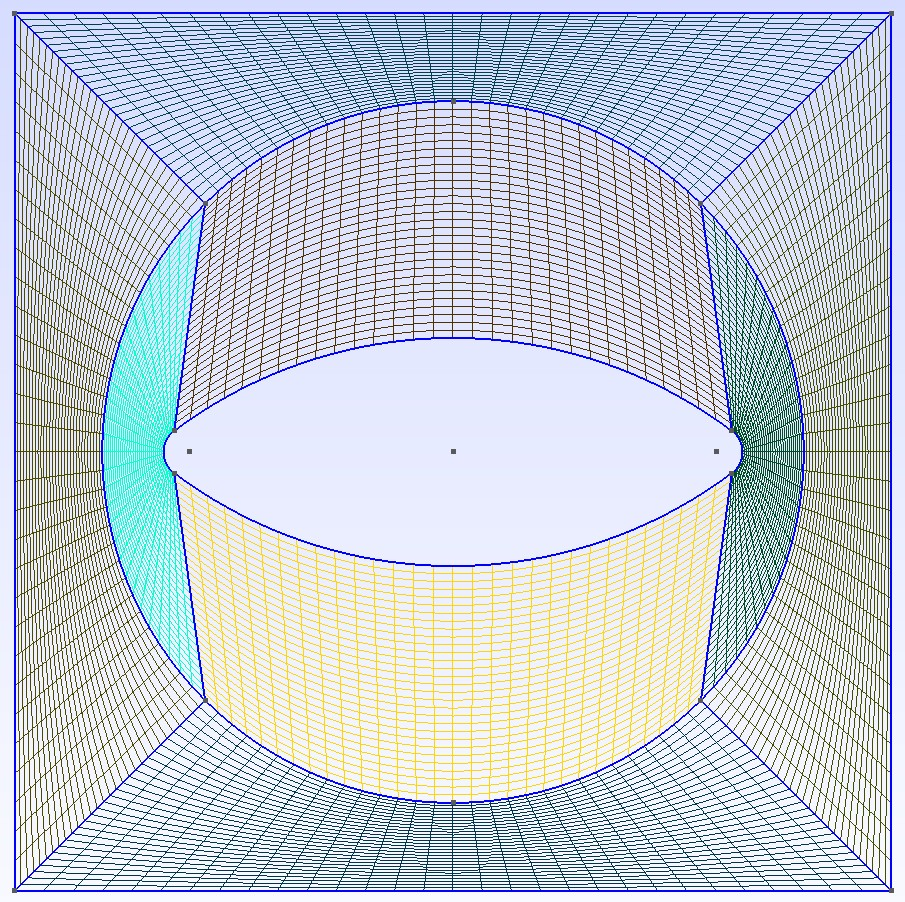
\includegraphics[width=0.3\linewidth]{alilk2.jpg}
    \caption{The Eye in Box (gradak2.msh)}
\end{figure}
\subsection{Input Equations}
\begin{itemize}
    \item $q = \sqrt{x^{2}+y^{2}}$: This equation is selected since it was given in the homework code itself. It is used to calculate the $L_2$ norm in all of the test meshes to get comparative results. 
    \item $q = {x^{2}+y^{2}}$: This is the previous equation without square root operator. This is selected since it was well defined in all boundaries.
    \item $q = cos{(x^{2}+y^{2})}$: This equation is selected to see whether the code implemented works for trigonometric functions or not. $Cos$ is selected on purpose since it is symmetric concerning the y-axis.
    \item $q = {x^{32}+y^{32}}$: This high-order function is selected for testing the limits of the code. Since it results in high numbers both numeric errors and method errors are enlarged.  
\end{itemize}
\subsection{$L_2$ Error Norms}
Note that the results calculate the $L_2$ error separately for each type of element. As a result, there are more than one result for meshes with more than one type of element. Furthermore, the results are reported in the format of [[x],[y]] with the first reported being triangular elements (if available) while the second line reports the quadrilateral elements (again, if available). 
\subsection{Results with Neumann Type Boundary Conditions}
Neumann boundary condition enforces no flux at boundaries which means that in the boundaries there is a "pretend" element with the same value of the left element. With no flux at the boundaries, Neumann-type boundary conditions allow for easy test case setup.\\\par 
Furthermore, the Neumann boundary condition eliminates the errors obtained during the boundary flux calculation phase of the test-case generation.\\\par
The results are tabulated below and on the next pages in tables 1 to 4: \\\par
\label{T1}
\begin{table}[H]
    \renewcommand\baselinestretch{1.1}\selectfont
    \centering
    \mbox{}\clap{
    \begin{tblr}
        []{
        rowsep = 0.5mm,
        colspec = {Q[c,m, 2cm]Q[c,m,4.7cm]Q[c,m,4.7cm]Q[c,m,4.7cm]},
        vlines, hlines}
        Mesh & $L_2$ Error Norm (GG) & $L_2$ Error Norm (LSQ) & $L_2$ Error Norm (wLSQ)  \\
       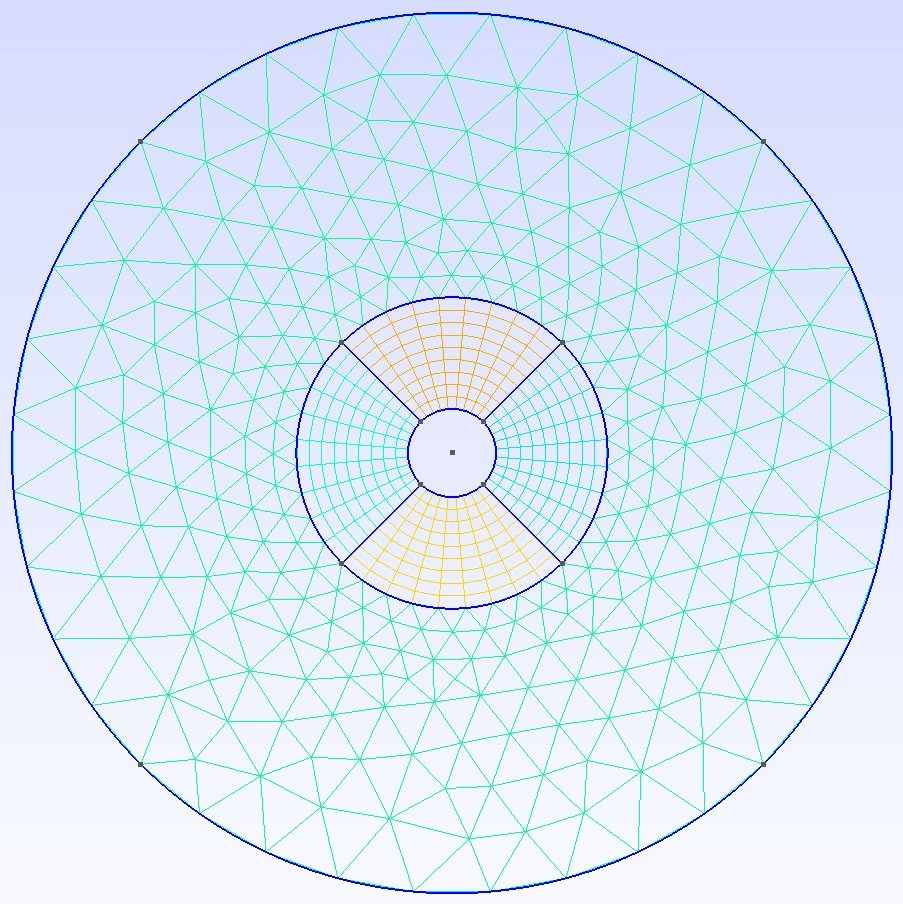
\includegraphics[width=0.4\linewidth, align=c]{grad.jpg} Figure 1 & {[[0.00240548],[0.00241336]]\newline[[0.07336319],[0.07294885]]} & {[[0.00246433],[0.00246418]]\newline[[0.06826314],[0.06729497]]} & {[[0.00239596],[0.00239596]]\newline[[0.06806001],[0.06765304]]}\\
       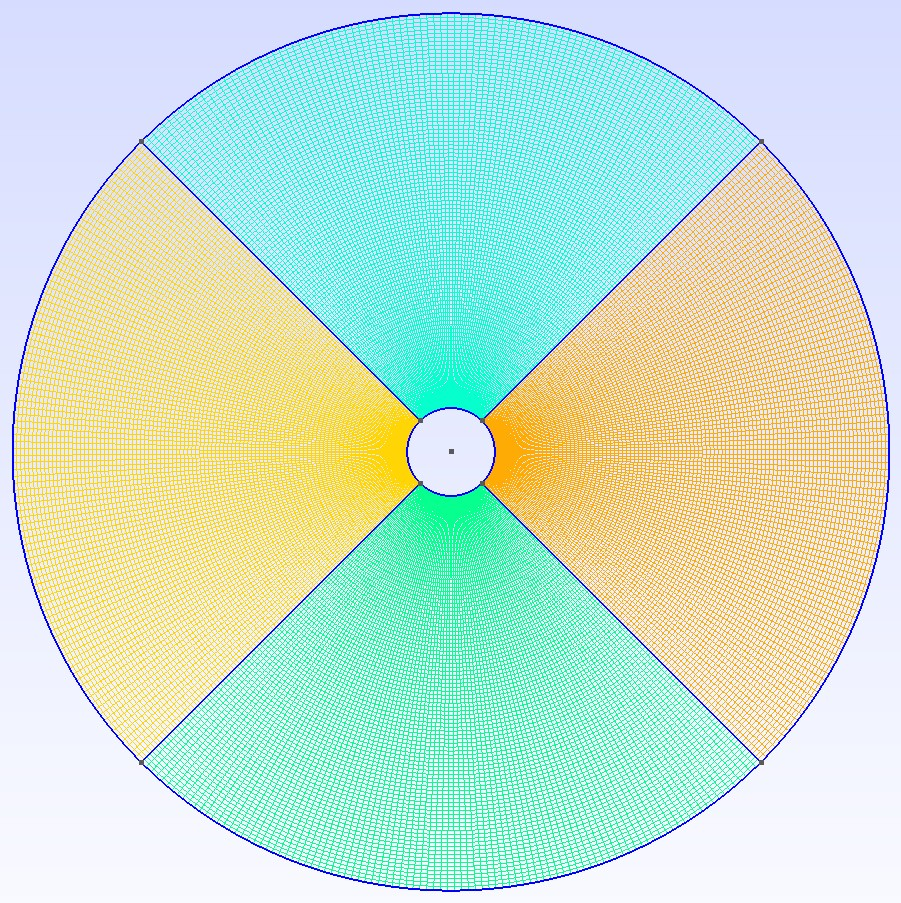
\includegraphics[width=0.4\linewidth, align=c]{grads.jpg} Figure 2 & [[0.0020397],[0.0020397]] & [[0.00203185],[0.00203185]] & [[0.0020316],[0.0020316]] \\
        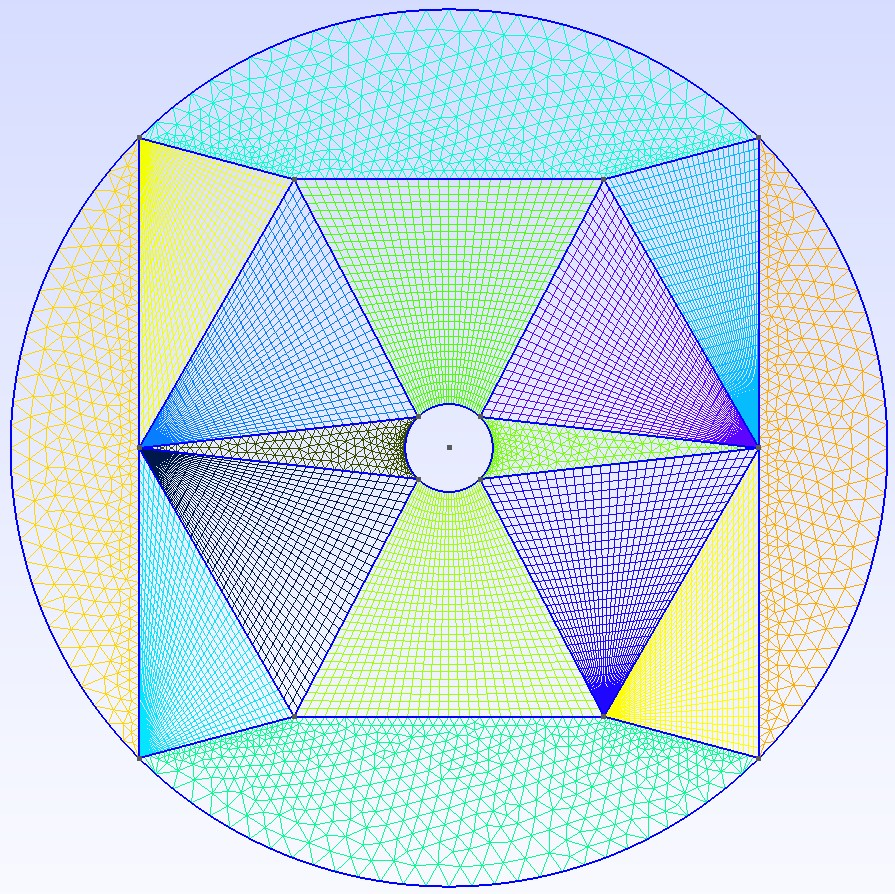
\includegraphics[width=0.4\linewidth, align=c]{onurk1.jpg} Figure 3 & {[[0.00210492],[0.00149657]]\newline[[0.01236622],[0.01227495]]} & {[[0.00082997],[0.00054637]]\newline[[0.01092133],[0.01090415]]} & {[[0.00036063],[0.00068709]]\newline[[0.01088902],[0.01081846]]} \\
        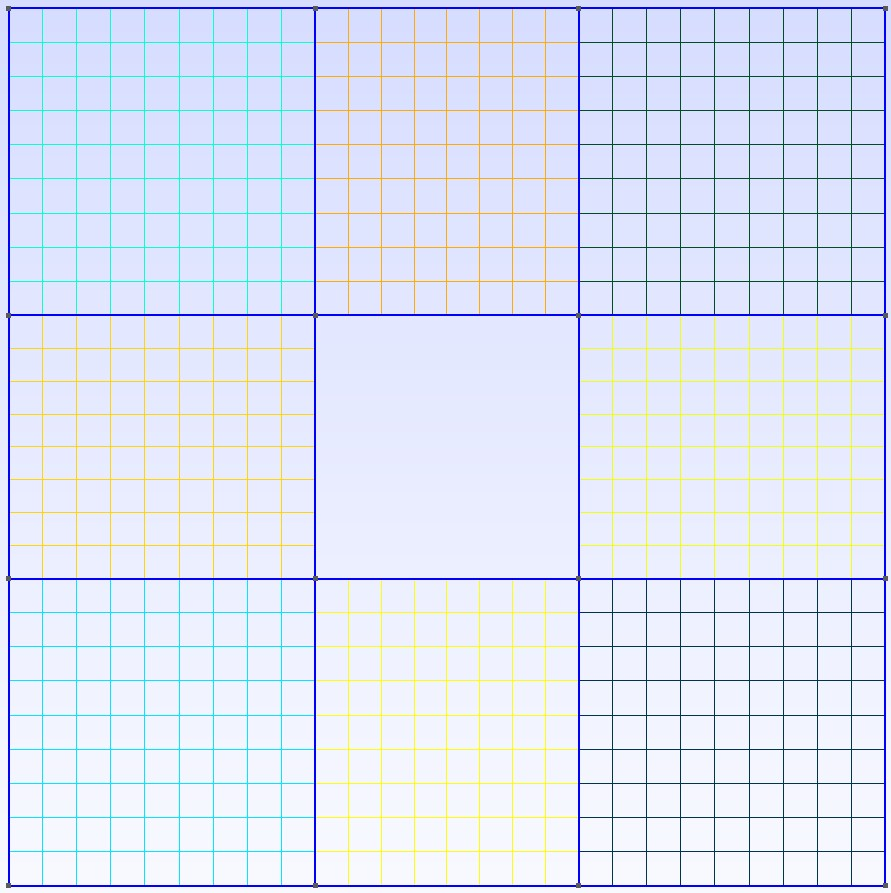
\includegraphics[width=0.4\linewidth, align=c]{onurk2.jpg} Figure 4 & [[0.0054402],[0.0054402]] & [[0.00543991],[0.00543991]] & [[0.00543995],[0.00543995]] \\
        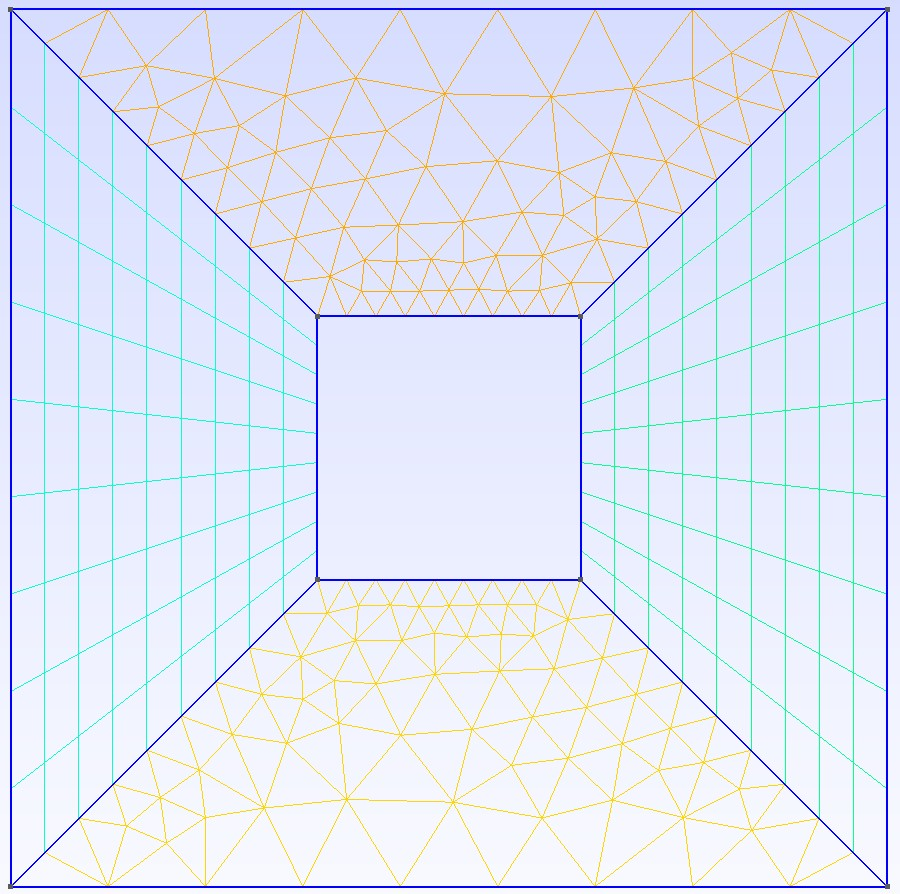
\includegraphics[width=0.4\linewidth, align=c]{onurk3.jpg} Figure 5 & {[[0.01048043],[0.00367857]]\newline[[0.00505206],[0.01158873]]} & {[[0.00818032],[0.00074892]]\newline[[0.0011861],[0.01094454]]} & {[[0.00926219],[0.00122]]\newline[[0.0009269],[0.0109231]]}\\
        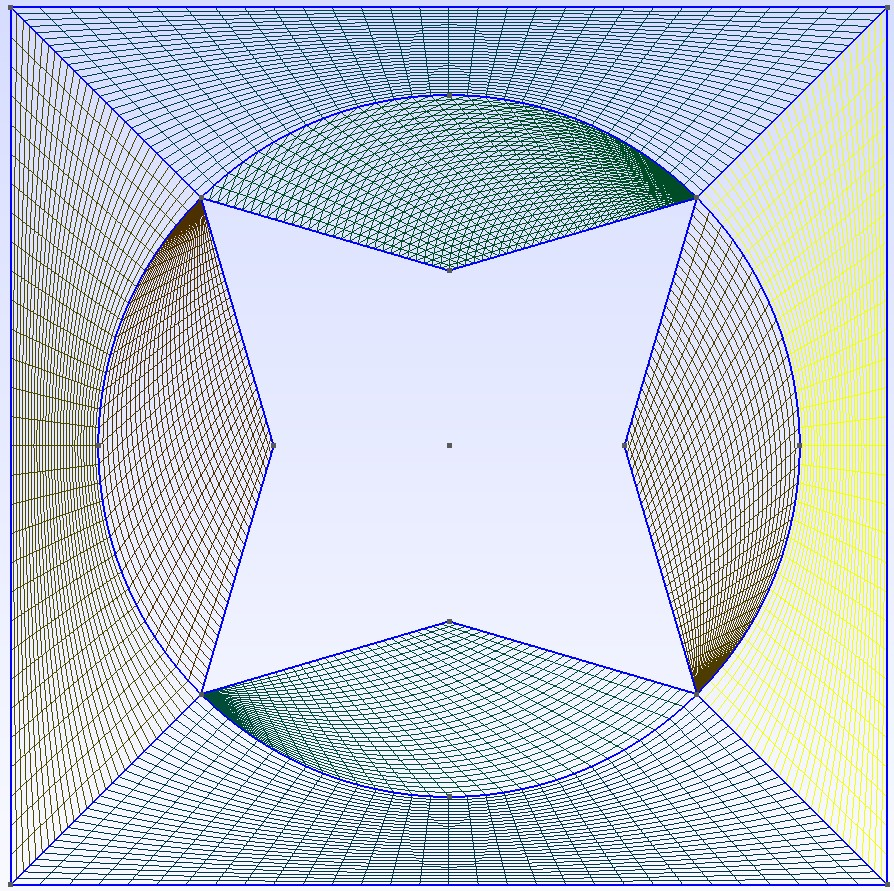
\includegraphics[width=0.4\linewidth, align=c]{alikmesh1.jpg} Figure 6 & {[[0.10761094],[0.10719521]]\newline[[0.01001063],[0.01608607]]} & {[[0.06580105],[0.05884946]]\newline[[0.00266881],[0.01688081]]} & {[[0.08054357],[0.0738357]]\newline[[0.00425521],[0.01401713]]}\\
        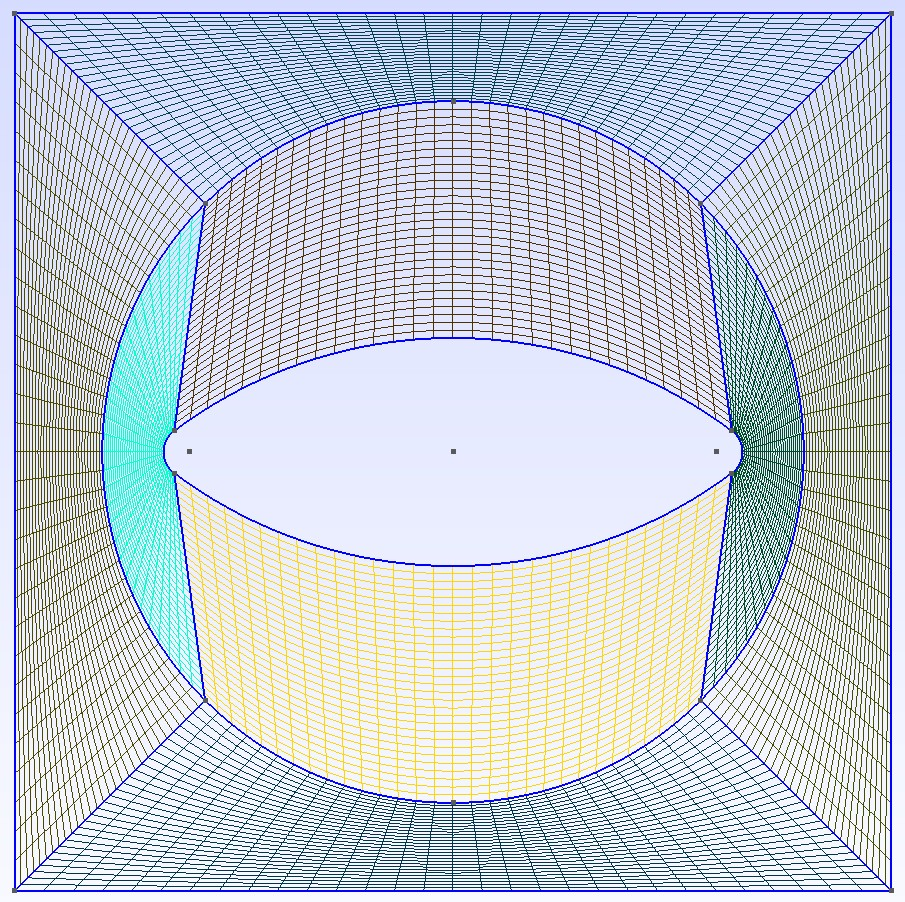
\includegraphics[width=0.4\linewidth, align=c]{alilk2.jpg} Figure 7 & [[0.10955121],[0.11720963]] & [[0.05365295],[0.07589494]] & [[0.07224261],[0.08830517]] \\
    \end{tblr}
    }
    \caption{Results for $q = \sqrt{x^2+y^2}$ Neumann}
\end{table}
\begin{table}[H]
    \renewcommand\baselinestretch{1.1}\selectfont
    \centering
    \mbox{}\clap{
    \begin{tblr}
        []{
        rowsep = 0.5mm,
        colspec = {Q[c,m, 2cm]Q[c,m,4.7cm]Q[c,m,4.7cm]Q[c,m,4.7cm]},
        vlines, hlines}
        Mesh & $L_2$ Error Norm (GG) & $L_2$ Error Norm (LSQ) & $L_2$ Error Norm (wLSQ)  \\
       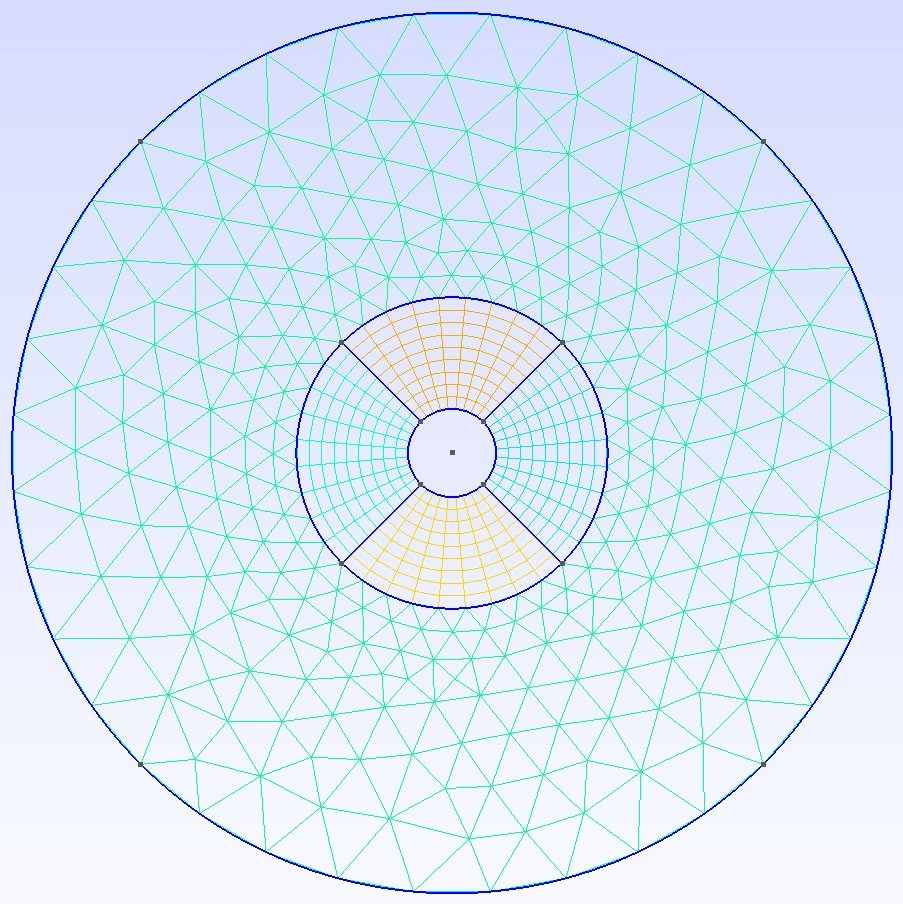
\includegraphics[width=0.4\linewidth, align=c]{grad.jpg} Figure 1 & {[[0.00140965],[0.00142458]]\newline[[0.19672191],[0.19469873]]} & {[[0.00083029],[0.00082941]]\newline[[0.18514975],[0.1825498]]} & {[[0.00069086],[0.0006908]]\newline[[0.18469784],[0.18361626]]}\\
       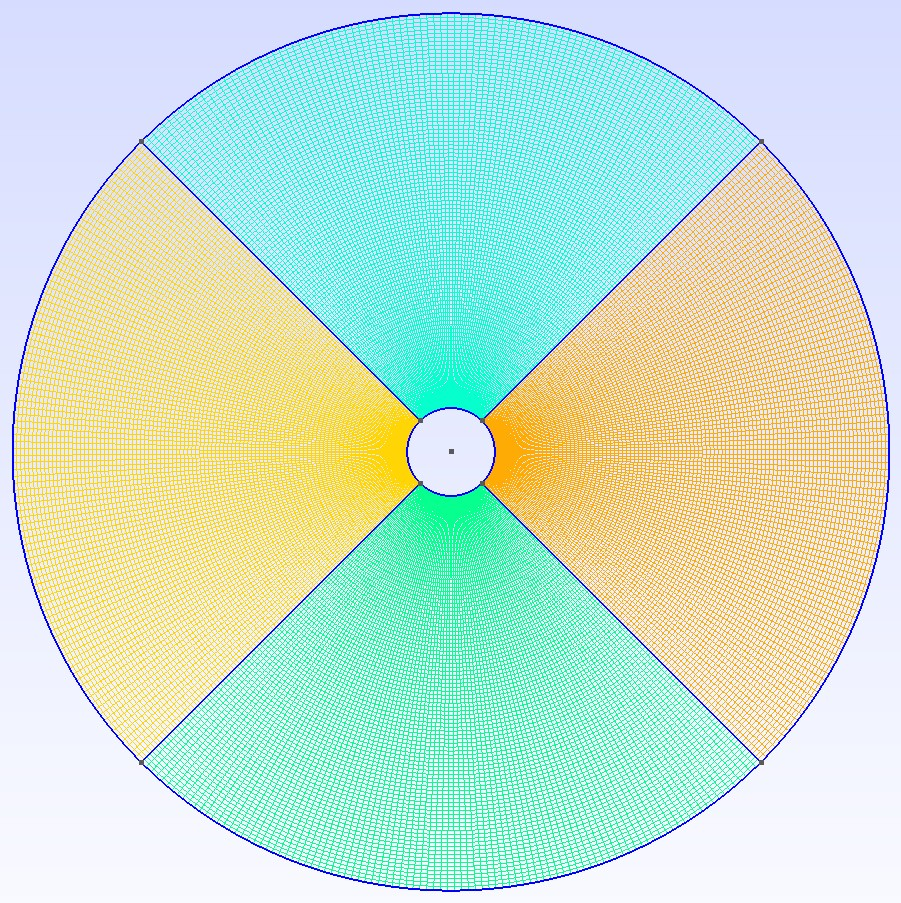
\includegraphics[width=0.4\linewidth, align=c]{grads.jpg} Figure 2 & [[0.00574039],[0.00574039]] & [[0.00571564],[0.00571564]] & [[0.00571492],[0.00571492]] \\
        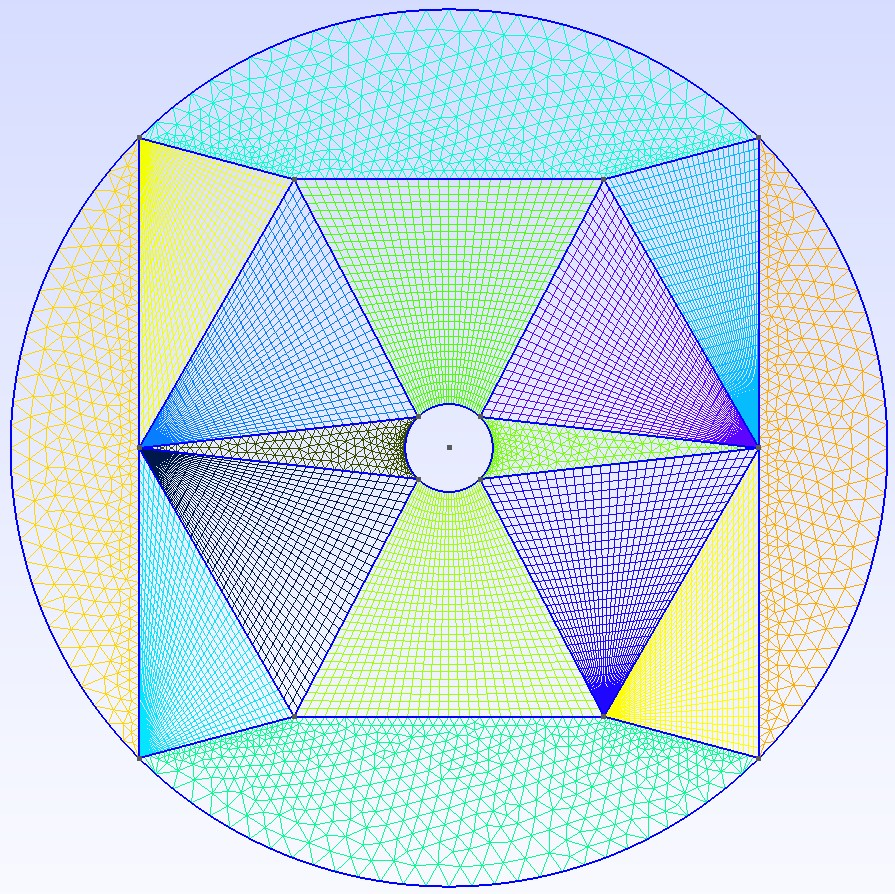
\includegraphics[width=0.4\linewidth, align=c]{onurk1.jpg} Figure 3 & {[[0.00390851],[0.00229017]]\newline[[0.03404243],[0.03366623]]} & {[[0.00028672],[0.00019171]]\newline[[0.0305426],[0.03048732]]} & {[[0.00011725],[0.00020285]]\newline[[0.03045901],[0.03025583]]} \\
        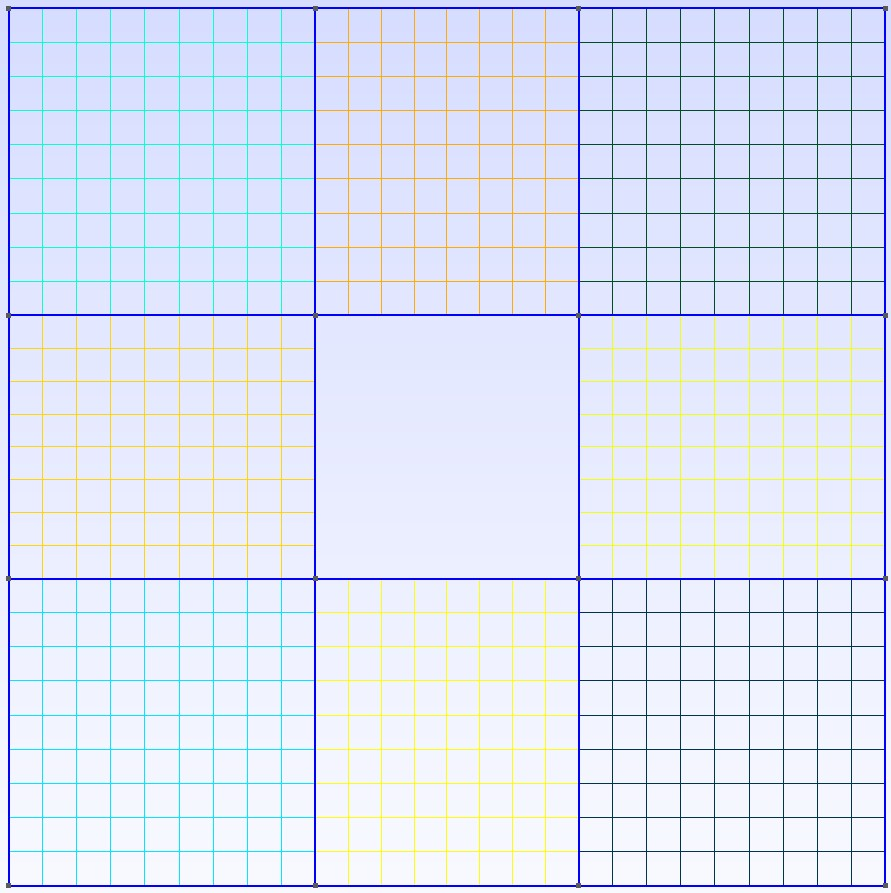
\includegraphics[width=0.4\linewidth, align=c]{onurk2.jpg} Figure 4 & [[0.00546429],[0.00546429]] & [[0.0054642],[0.0054642]] & [[0.00546418],[0.00546418]] \\
        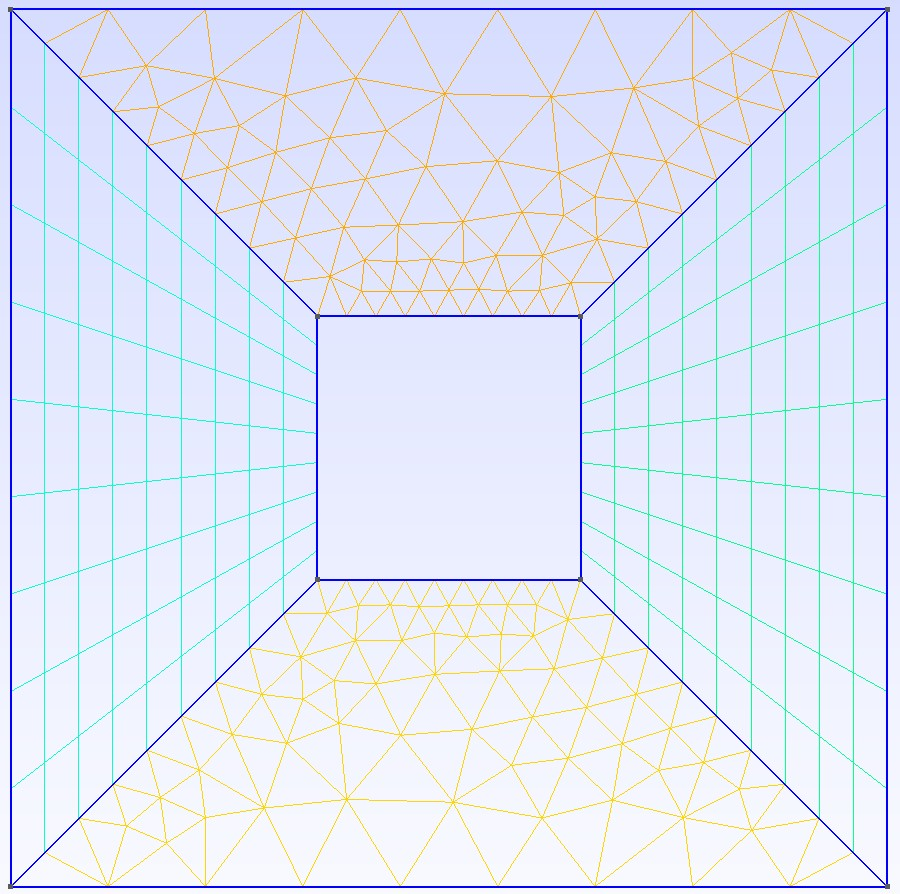
\includegraphics[width=0.4\linewidth, align=c]{onurk3.jpg} Figure 5 & {[[0.01146731],[0.00422454]]\newline[[0.00523682],[0.01167767]]} & {[[0.00873108],[0.00089568]]\newline[[0.00096221],[0.0110435]]} & {[[0.0100125],[0.00128757]]\newline[[0.00078837],[0.01112919]]}\\
        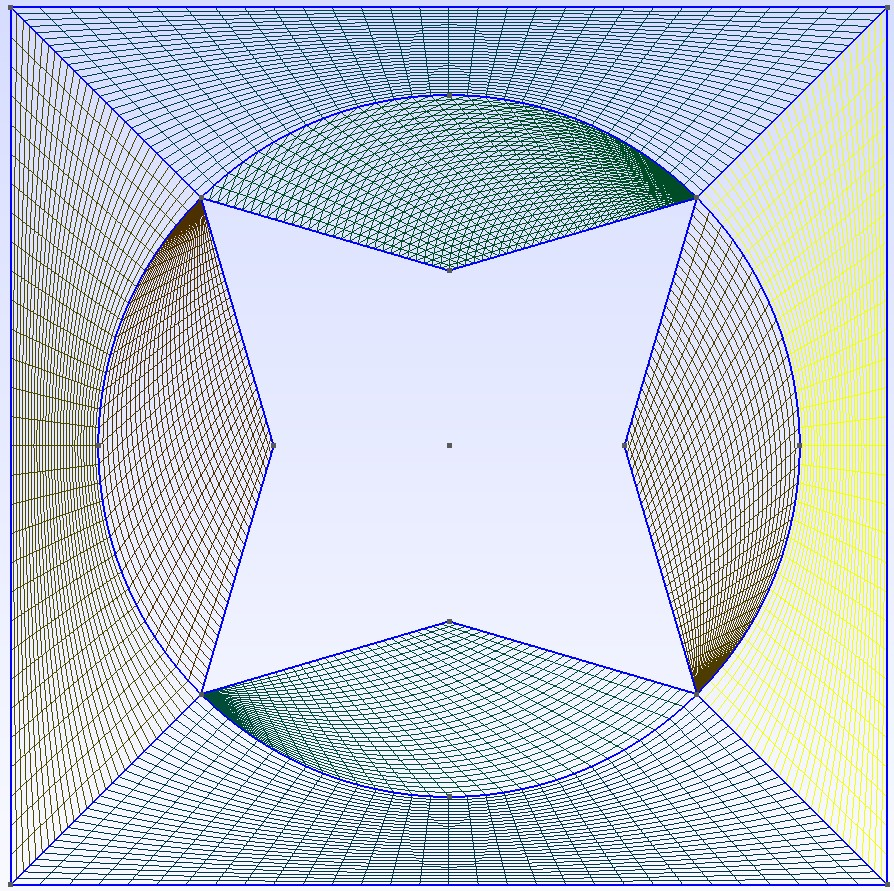
\includegraphics[width=0.4\linewidth, align=c]{alikmesh1.jpg} Figure 6 & {[[1.31401775],[1.31253684]]\newline[[0.07762136],[0.11023263]]} & {[[0.64263714],[0.61776353]]\newline[[0.01468941],[0.10029174]]} & {[[0.83643376],[0.8160706]]\newline[[0.02239149],[0.0772916]]}\\
        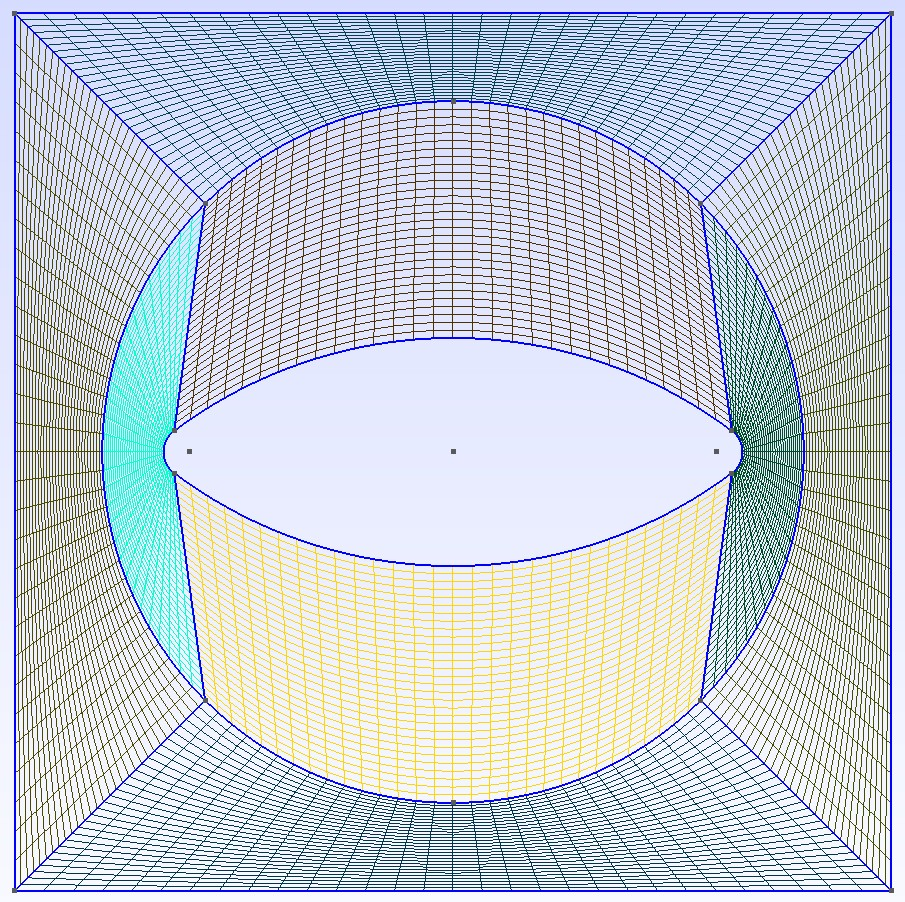
\includegraphics[width=0.4\linewidth, align=c]{alilk2.jpg} Figure 7 & [[1.31916359],[1.32371419]] & [[0.59665498],[0.62363335]] & [[0.80742175],[0.8235998]] \\
    \end{tblr}
    }
    \caption{Results for $q = x^2+y^2$ Neumann}
\end{table}
\label{T3}
\begin{table}[H]
    \renewcommand\baselinestretch{1.1}\selectfont
    \centering
    \mbox{}\clap{
    \begin{tblr}
        []{
        rowsep = 0.5mm,
        colspec = {Q[c,m, 2cm]Q[c,m,4.7cm]Q[c,m,4.7cm]Q[c,m,4.7cm]},
        vlines, hlines}
        Mesh & $L_2$ Error Norm (GG) & $L_2$ Error Norm (LSQ) & $L_2$ Error Norm (wLSQ)  \\
       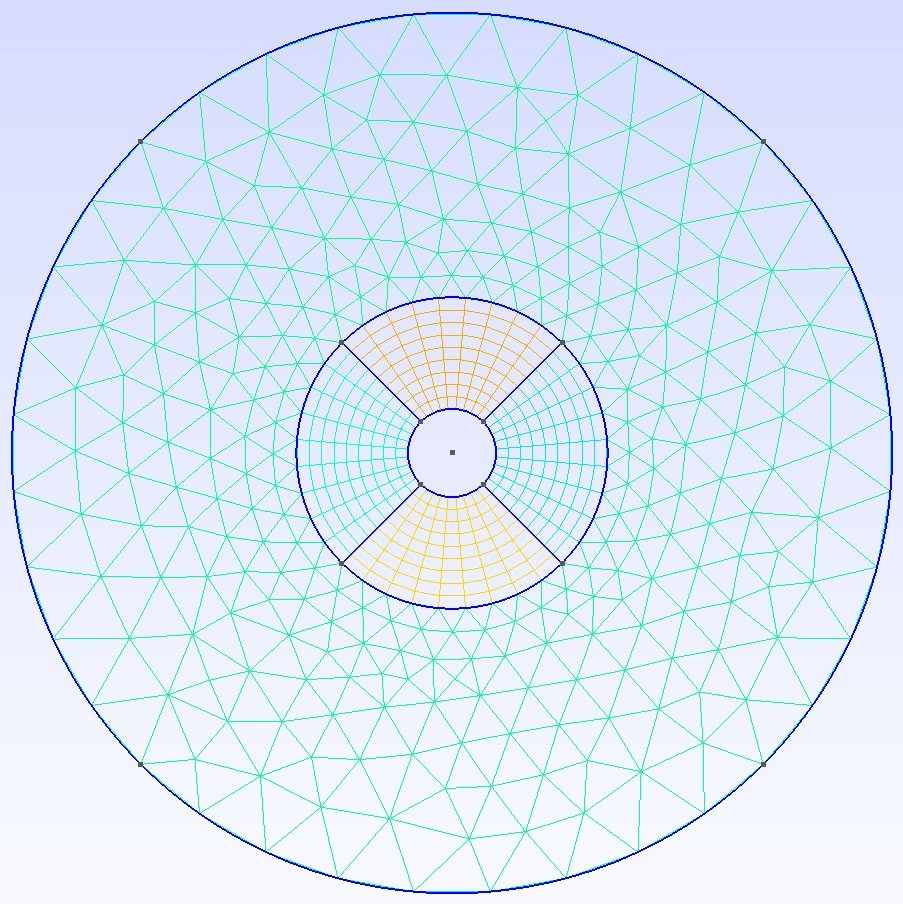
\includegraphics[width=0.4\linewidth, align=c]{grad.jpg} Figure 1 & {[[0.00037888],[0.00038329]]\newline[[0.19058115],[0.18828494]]} & {[[6.5388e-05],[6.5793e-05]]\newline[[0.17906887],[0.17648487]]} & {[[3.5068e-05],[3.5340e-05]]\newline[[0.17853048],[0.17742921]]}\\
       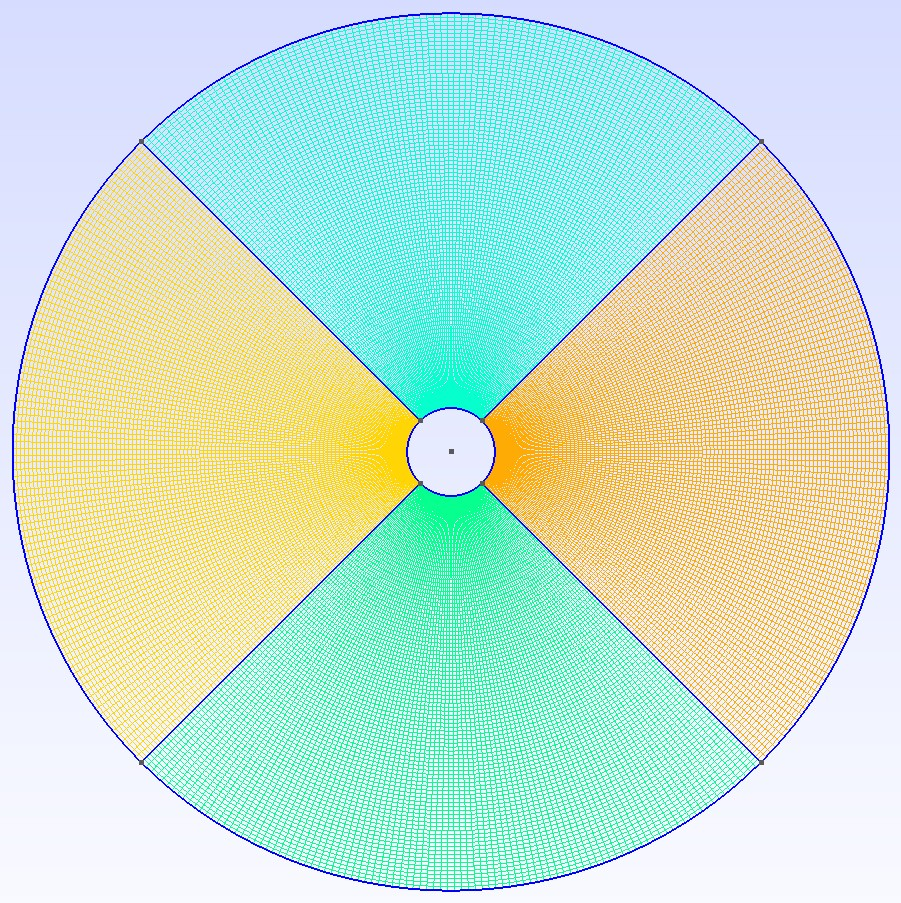
\includegraphics[width=0.4\linewidth, align=c]{grads.jpg} Figure 2 & [[0.00522279],[0.00522279]] & [[0.00519991],[0.00519991]] & [[0.00519924],[0.00519924]] \\
        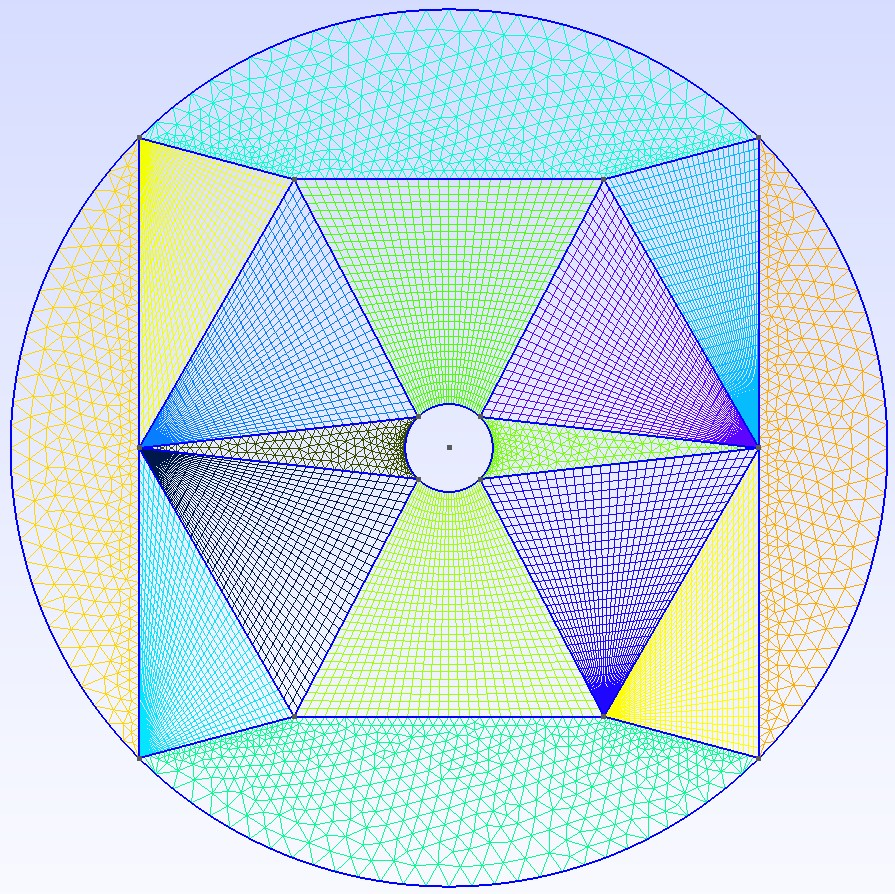
\includegraphics[width=0.4\linewidth, align=c]{onurk1.jpg} Figure 3 & {[[0.00323153],[0.00179723]]\newline[[0.03178523],[0.03142236]]} & {[[0.00011116],[0.00012576]]\newline[[0.02831751],[0.02827726]]} & {[[7.5896e-05],[6.4593e-05]]\newline[[0.02823049],[0.02805004]]} \\
        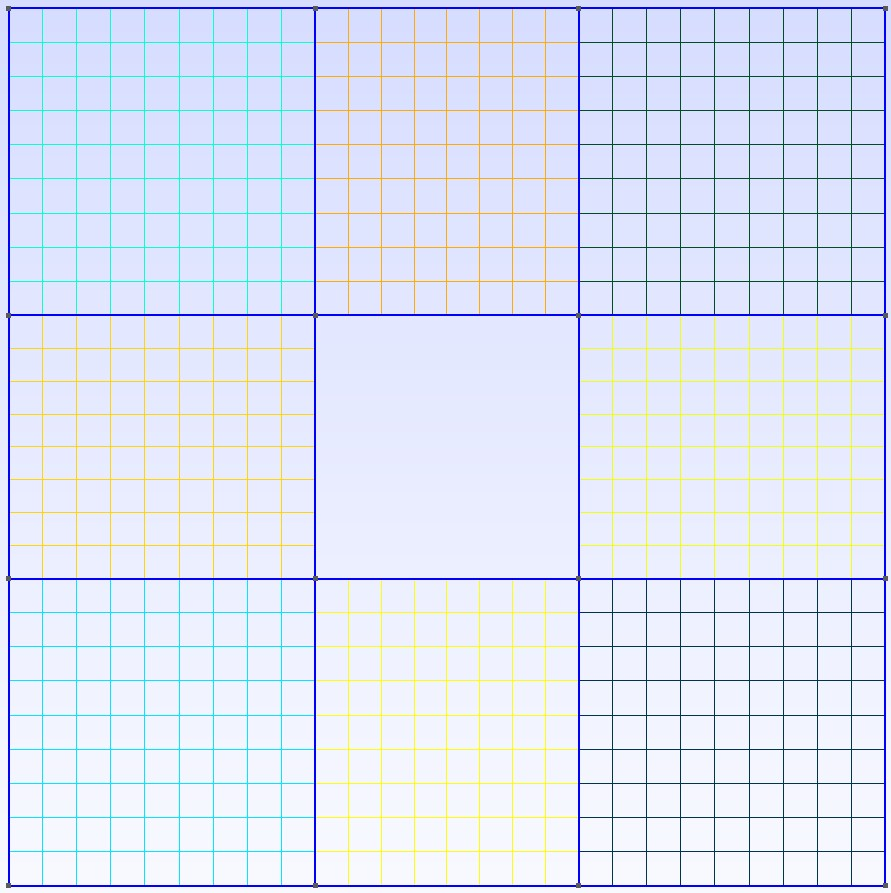
\includegraphics[width=0.4\linewidth, align=c]{onurk2.jpg} Figure 4 & [[0.00179106],[0.00179106]] & [[0.00179106],[0.00179106]] & [[0.00179105],[0.00179105]] \\
        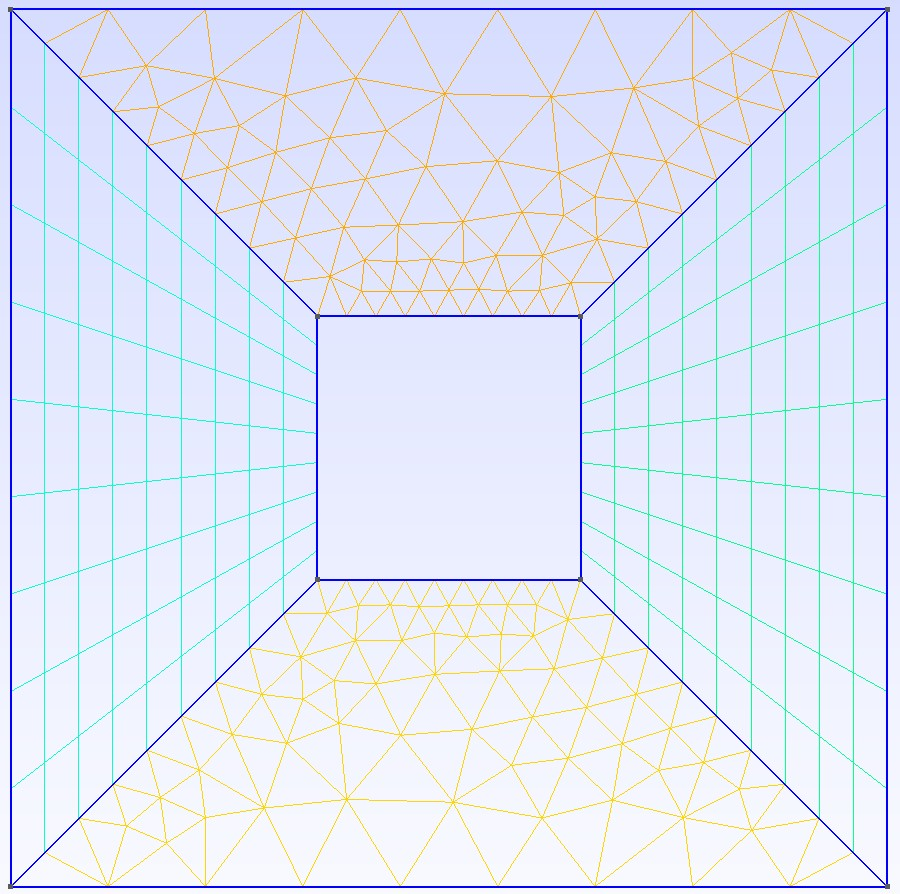
\includegraphics[width=0.4\linewidth, align=c]{onurk3.jpg} Figure 5 & {[[0.0038207],[0.00158006]]\newline[[0.00176743],[0.00313644]]} & {[[0.00290303],[0.00052983]]\newline[[0.00033844],[0.00293117]]} & {[[0.00334377],[0.00047014]]\newline[[0.00027598],[0.00304322]]}\\
        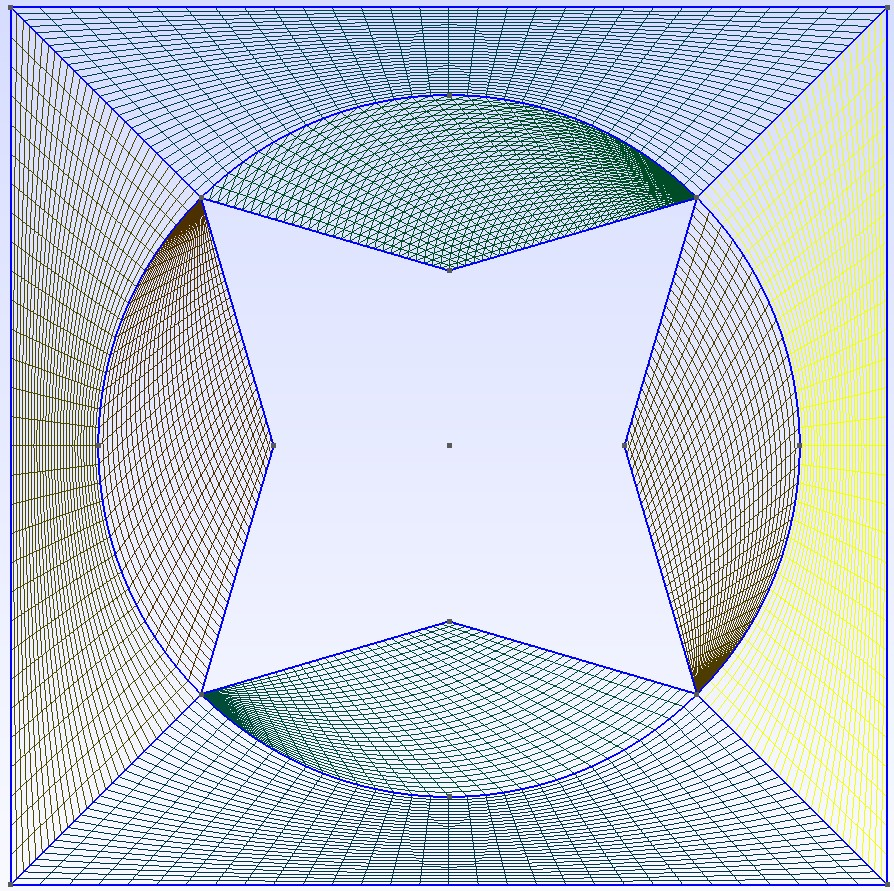
\includegraphics[width=0.4\linewidth, align=c]{alikmesh1.jpg} Figure 6 & {[[1.42608863],[1.42529982]]\newline[[0.06092356],[0.09625521]]} & {[[1.4520296 ],[1.44568491]]\newline[[0.04909822],[0.10070024]]} & {[[1.27655278],[1.26899789]]\newline[[0.05077559],[0.12243265]]}\\
        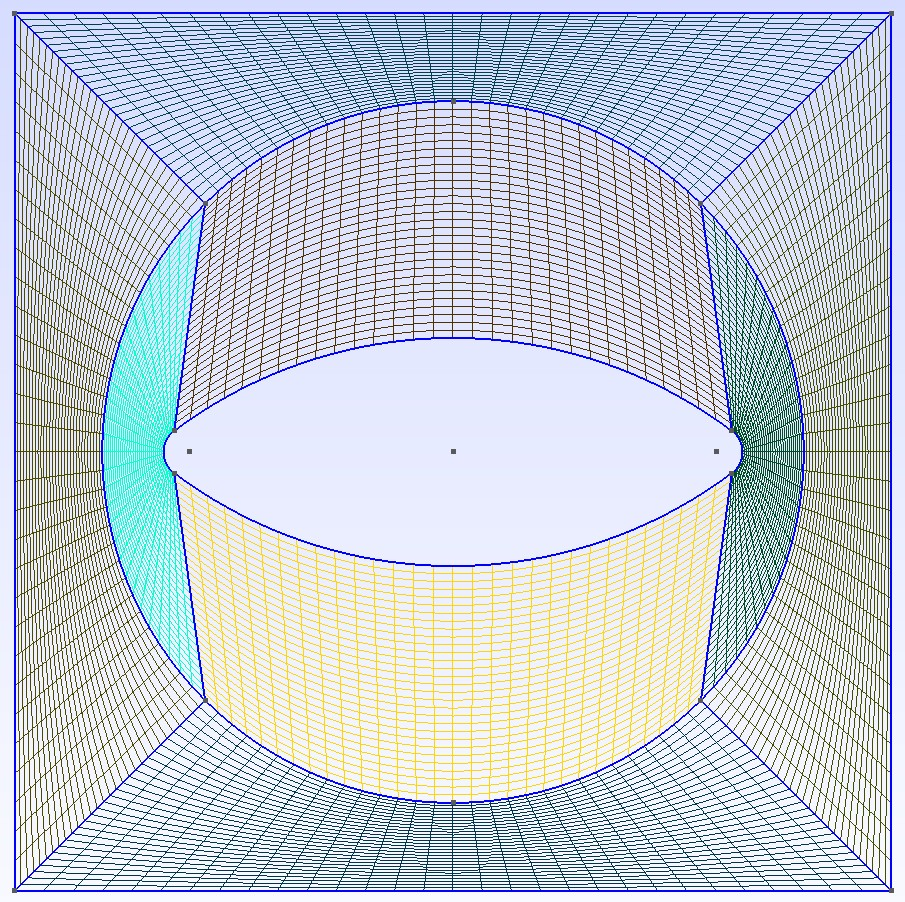
\includegraphics[width=0.4\linewidth, align=c]{alilk2.jpg} Figure 7 & [[1.43300951],[1.43431454]] & [[1.4486257],[1.45477046]] & [[1.27167525],[1.27577778]] \\
    \end{tblr}
    }
    \caption{Results for $q = cos(x^2+y^2)$ Neumann}
\end{table}
\begin{table}[H]
    \renewcommand\baselinestretch{1.1}\selectfont
    \centering
    \mbox{}\clap{
    \begin{tblr}
        []{
        rowsep = 0.5mm,
        colspec = {Q[c,m, 2cm]Q[c,m,4.7cm]Q[c,m,4.7cm]Q[c,m,4.7cm]},
        vlines, hlines}
        Mesh & $L_2$ Error Norm (GG) & $L_2$ Error Norm (LSQ) & $L_2$ Error Norm (wLSQ)  \\
       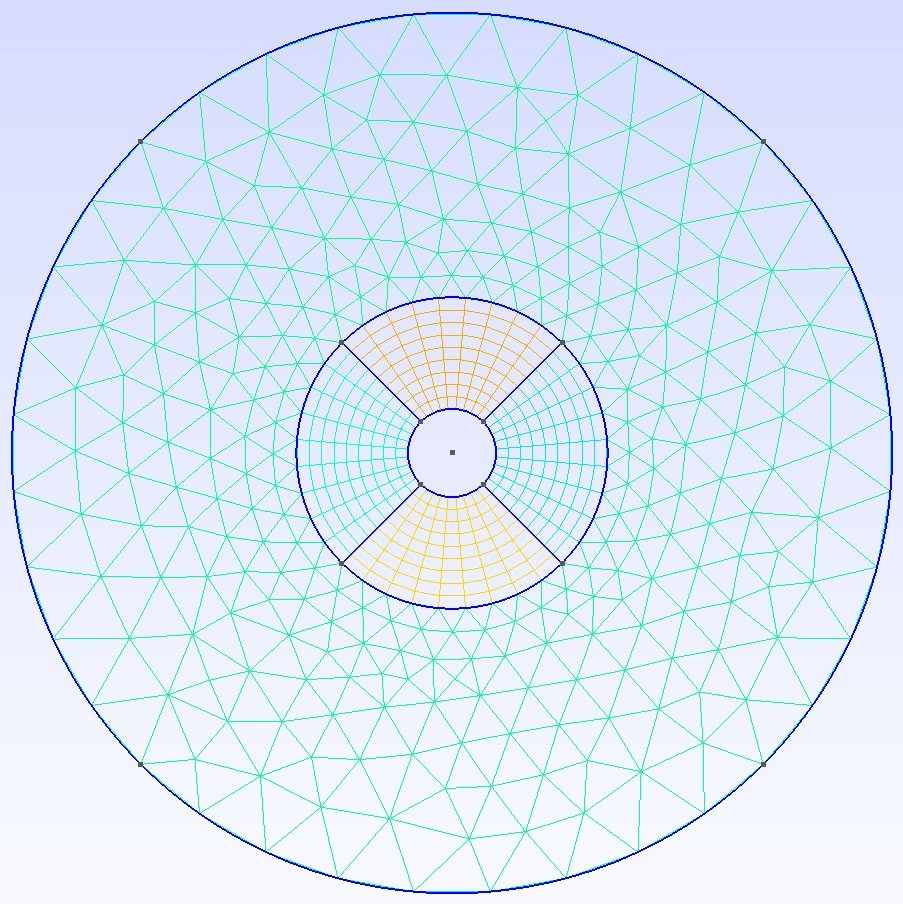
\includegraphics[width=0.4\linewidth, align=c]{grad.jpg} Figure 1 & {[[5.8831e-11],[5.9212e-11]]\newline[[11617.5792],[11598.3844]]} & {[[5.2688e-11],[5.3015e-11]]\newline[[11551.6226],[11511.8233]]} & {[[4.6176e-11],[4.6361e-11]]\newline[[11626.8597],[11741.9614]]}\\
       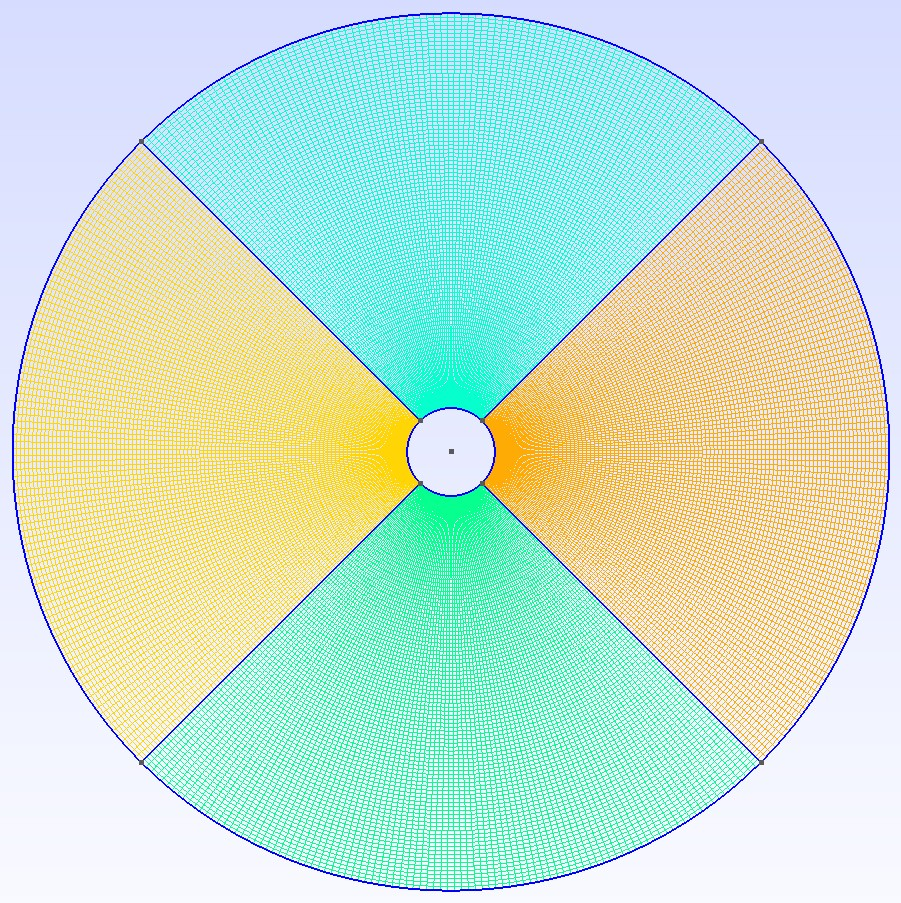
\includegraphics[width=0.4\linewidth, align=c]{grads.jpg} Figure 2 & [[1313.4353],[1313.4353]] & [[1308.8182],[1308.8182]] & [[1308.8435],[1308.8435]] \\
        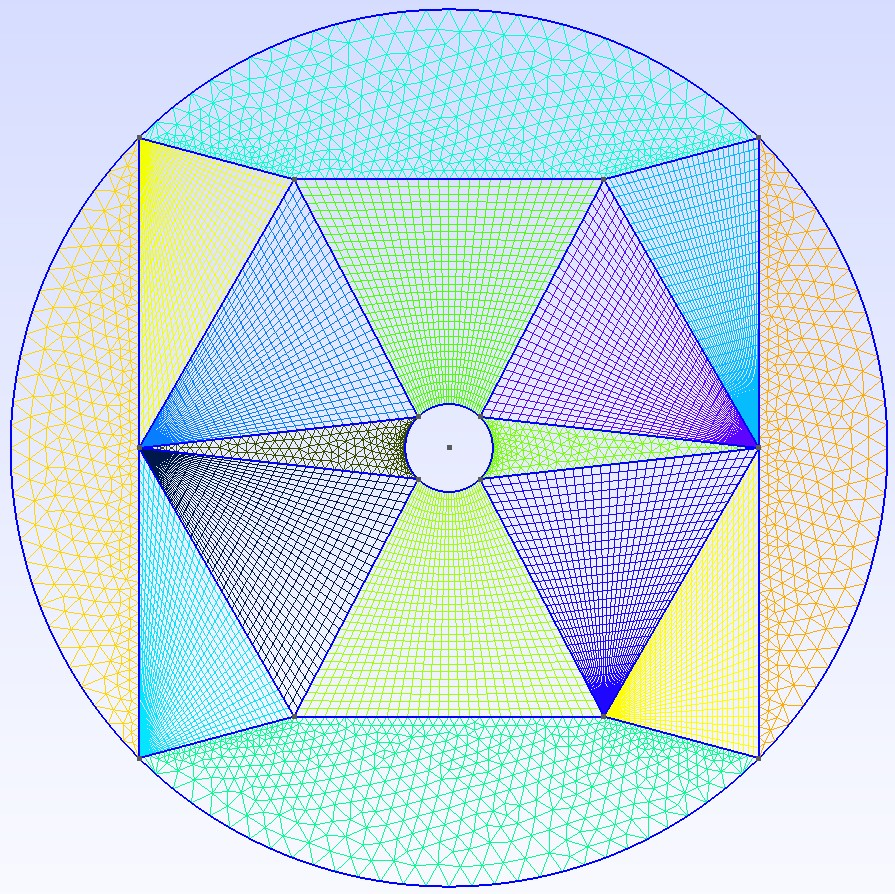
\includegraphics[width=0.4\linewidth, align=c]{onurk1.jpg} Figure 3 & {[[0.04038635],[0.00961823]]\newline[[5459.4218],[5675.2439]]} & {[[0.01646438],[0.00522647]]\newline[[5403.7340],[5582.2484]]} & {[[0.01743961],[0.00520740]]\newline[[5424.7127],[5533.0589]]} \\
        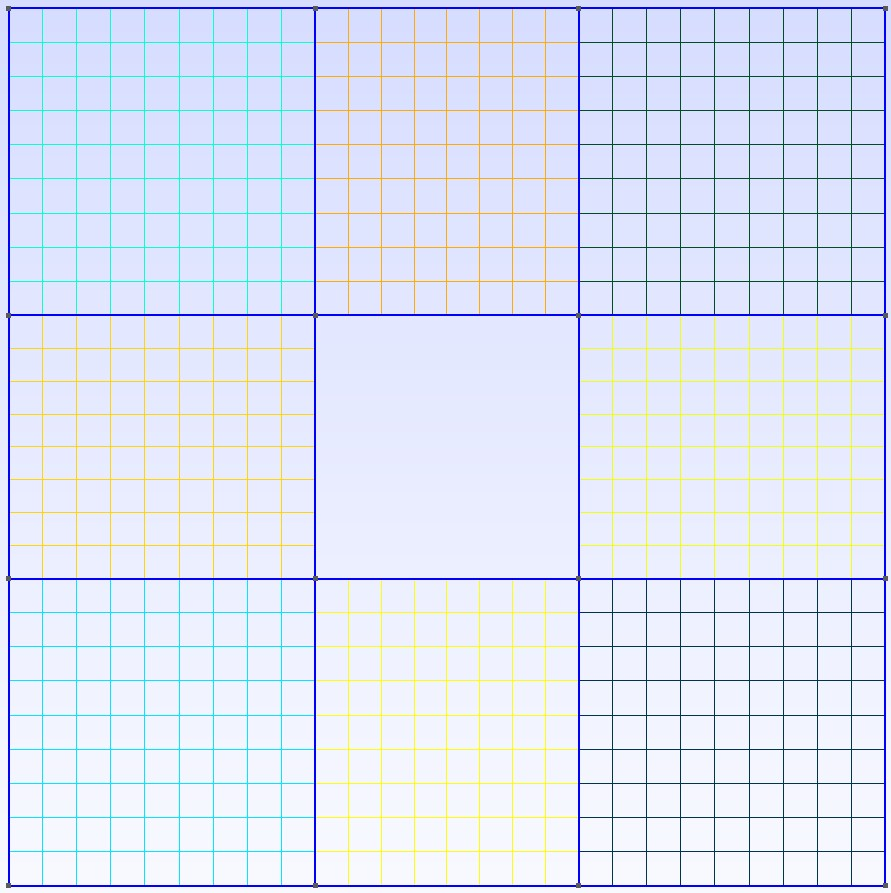
\includegraphics[width=0.4\linewidth, align=c]{onurk2.jpg} Figure 4 & [[3.8944e-11],[3.8944e-11]] & [[3.8944e-11],[3.8944e-11]] & [[3.8944e-11],[3.8944e-11]] \\
        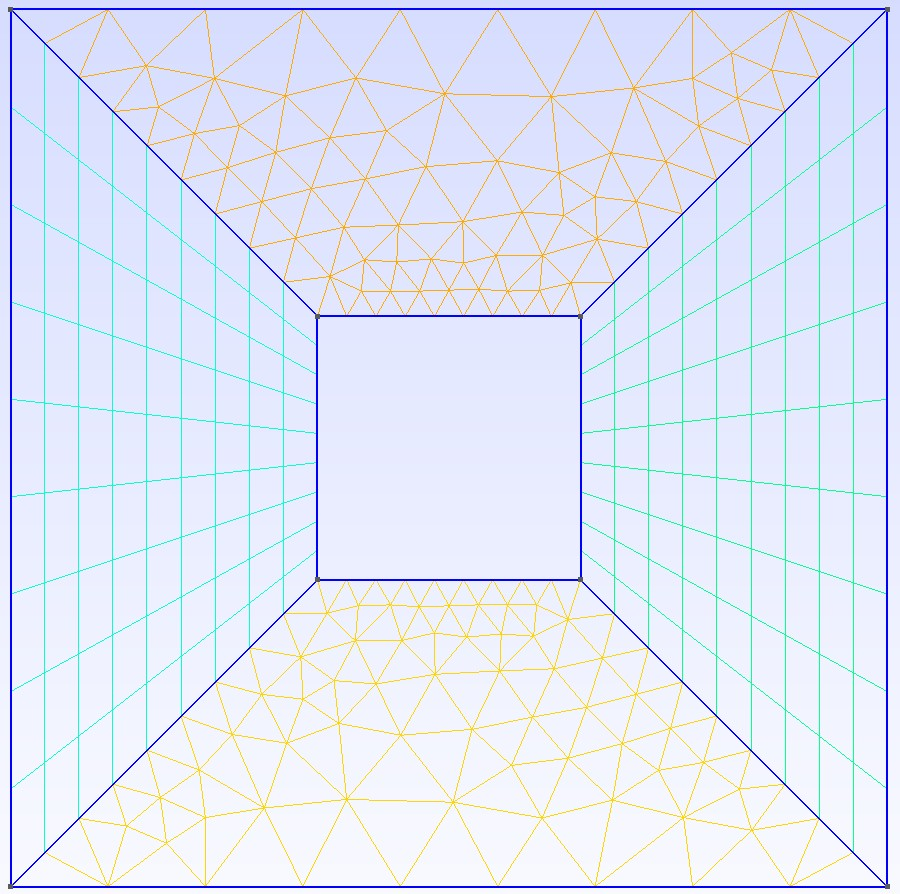
\includegraphics[width=0.4\linewidth, align=c]{onurk3.jpg} Figure 5 & {[[6.4849e-11],[8.8478e-13]]\newline[[6.0220e-12],[4.2501e-11]]} & {[[6.5355e-11],[1.9387e-12]]\newline[[7.5760e-12],[4.3563e-11]]} & {[[6.6582e-11],[4.8111e-12]]\newline[[7.8197e-12],[4.5038e-11]]}\\
        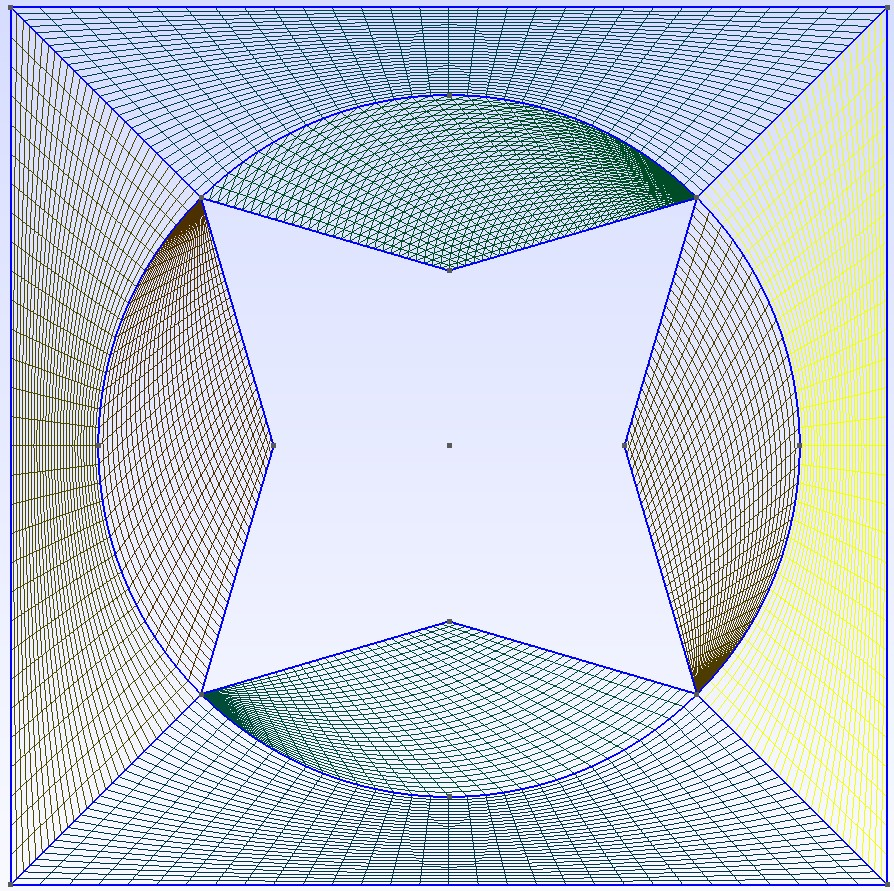
\includegraphics[width=0.4\linewidth, align=c]{alikmesh1.jpg} Figure 6 & {[[9.3061e+21],[9.3061e+21]]\newline[[1.0466e+17],[2.8341e+17]]} & {[[9.7141e+21],[9.7141e+21]]\newline[[1.0106e+17],[2.2595e+17]]} & {[[1.1158e+22],[1.1158e+22]]\newline[[9.5219e+16],[3.8537e+17]]}\\
        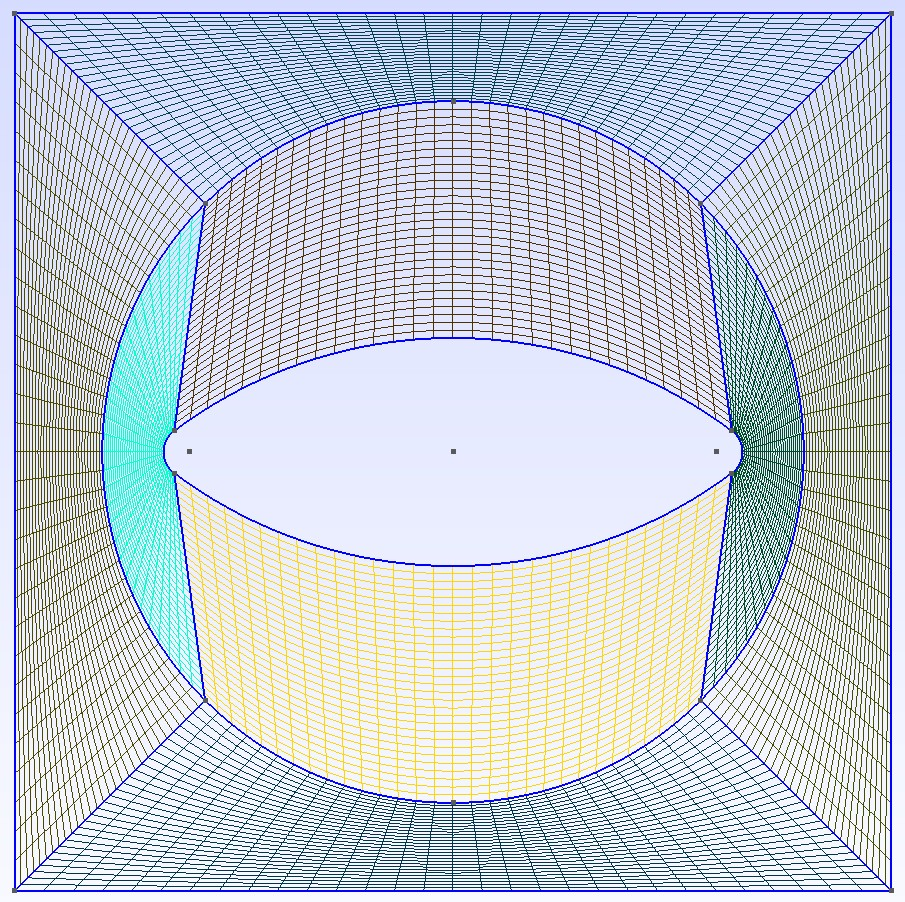
\includegraphics[width=0.4\linewidth, align=c]{alilk2.jpg} Figure 7 & [[9.3061e+21],[9.3061e+21]] & [[9.7141e+21],[9.7141e+21]] & [[1.1158e+22],[1.1158e+22]] \\
    \end{tblr}
    }
    \caption{Results for $q = x^{32}+y^{32}$ Neumann}
\end{table}

\label{s7.5}
\subsection{Results with Drichlet Type Boundary Conditions} \label{drichlet}
These results were obtained by using the Drichlet condition. For the inner and outer fluxes the initial condition equation was evaluated at the location of the boundaries for uncommon shaped boundaries the equation was evaluated at different locations on the boundary and simply averaged to get a \verb|q| value.\\\par
This introduces a lot of error for uncommon boundary shapes and/or unsymmetrical variable equations. The error introduced is obvious when one compares the Drichlet boundary condition $L_2$ error norms of the same mesh with the Neumann boundary condition $L_2$ error norms.\\\par
The results are tabulated on the next pages in tables 5 to 8: \\\par
\begin{table}[H]
    \renewcommand\baselinestretch{1.1}\selectfont
    \centering
    \mbox{}\clap{
    \begin{tblr}
        []{
        rowsep = 0.5mm,
        colspec = {Q[c,m, 2cm]Q[c,m,4.7cm]Q[c,m,4.7cm]Q[c,m,4.7cm]},
        vlines, hlines}
        Mesh & $L_2$ Error Norm (GG) & $L_2$ Error Norm (LSQ) & $L_2$ Error Norm (wLSQ)  \\
       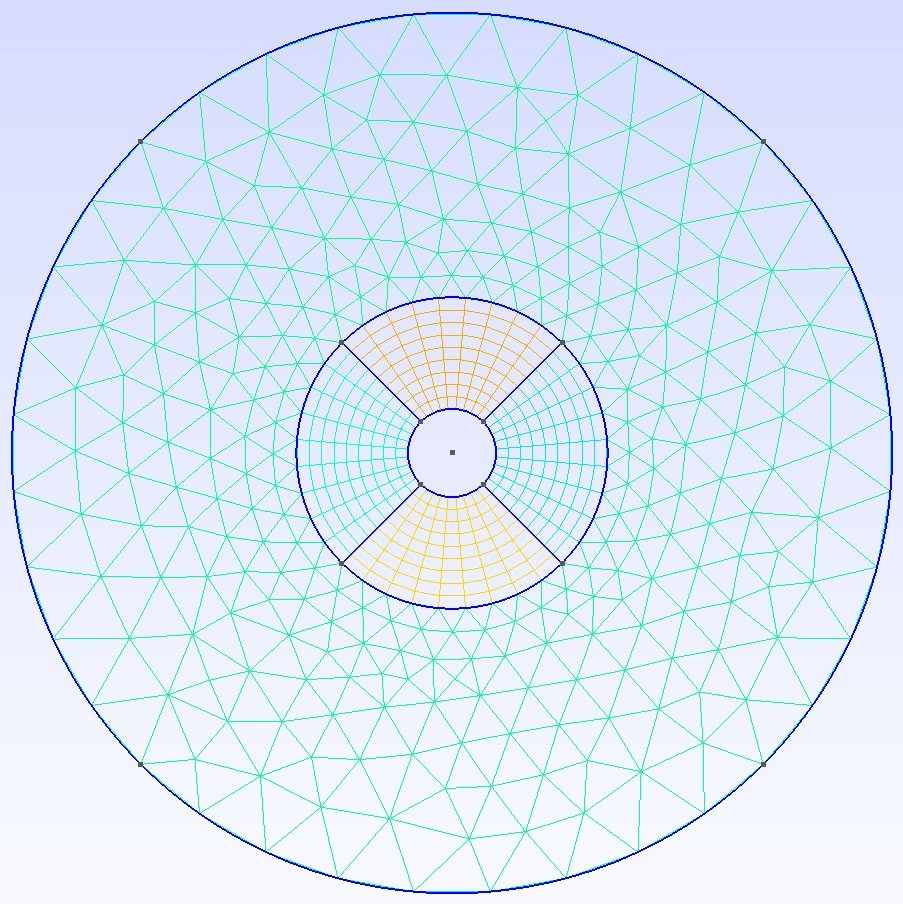
\includegraphics[width=0.4\linewidth, align=c]{grad.jpg} Figure 1 & {[[0.00161697],[0.00162867]]\newline[[0.04102047],[0.04169986]]} & {[[0.00139097],[0.00139071]]\newline[[0.03299403],[0.03254984]]} &{[[0.00126205],[0.00126205]] \newline[[0.03287267],[0.0326414]] }\\
       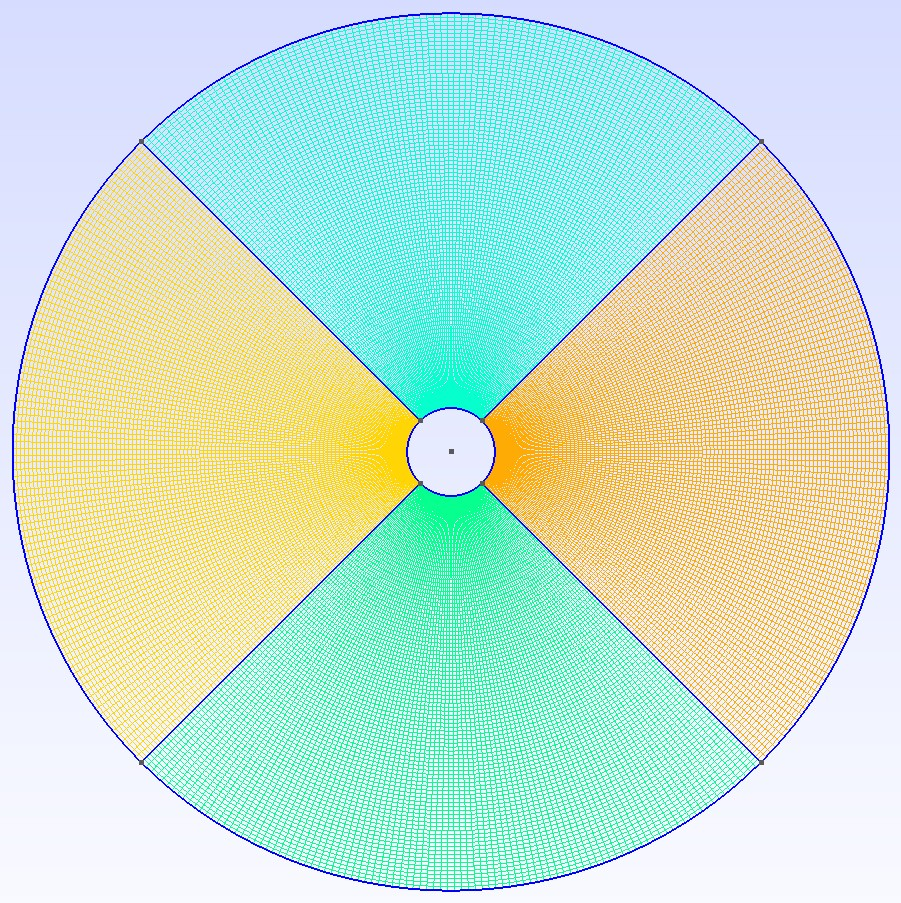
\includegraphics[width=0.4\linewidth, align=c]{grads.jpg} Figure 2 & {[[0.00101287],[0.00101287]]}   & [[0.00100936],[0.00100936]] & {[[0.00100898],[0.00100898]]} \\
        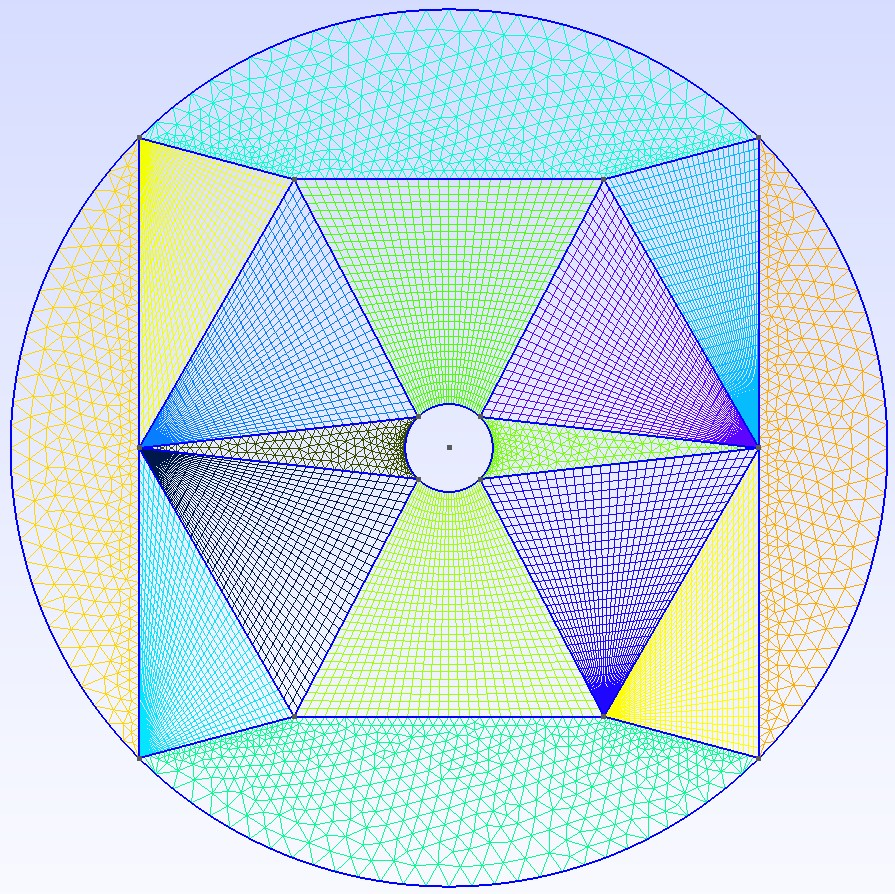
\includegraphics[width=0.4\linewidth, align=c]{onurk1.jpg} Figure 3 & {[[0.00209438],[0.00137893]]\newline[[0.00784781],[0.00788279]]} & {[[0.00042374],[0.00028083]]\newline[[0.00539358],[0.00538197]]} & {[[0.00018216],[0.00034561]]\newline[[0.00537691],[0.00533905]]} \\
        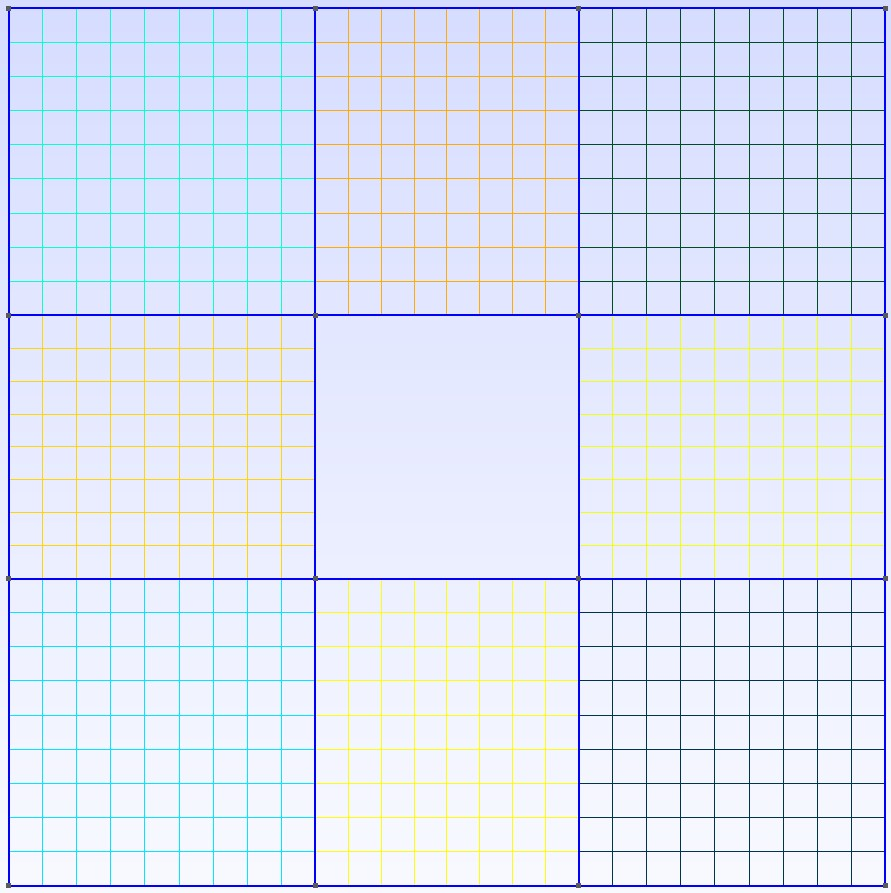
\includegraphics[width=0.4\linewidth, align=c]{onurk2.jpg} Figure 4 & [[0.0186705],[0.0186705]] & [[0.01867041],[0.01867041]] & [[0.01867042],[0.01867042]] \\
        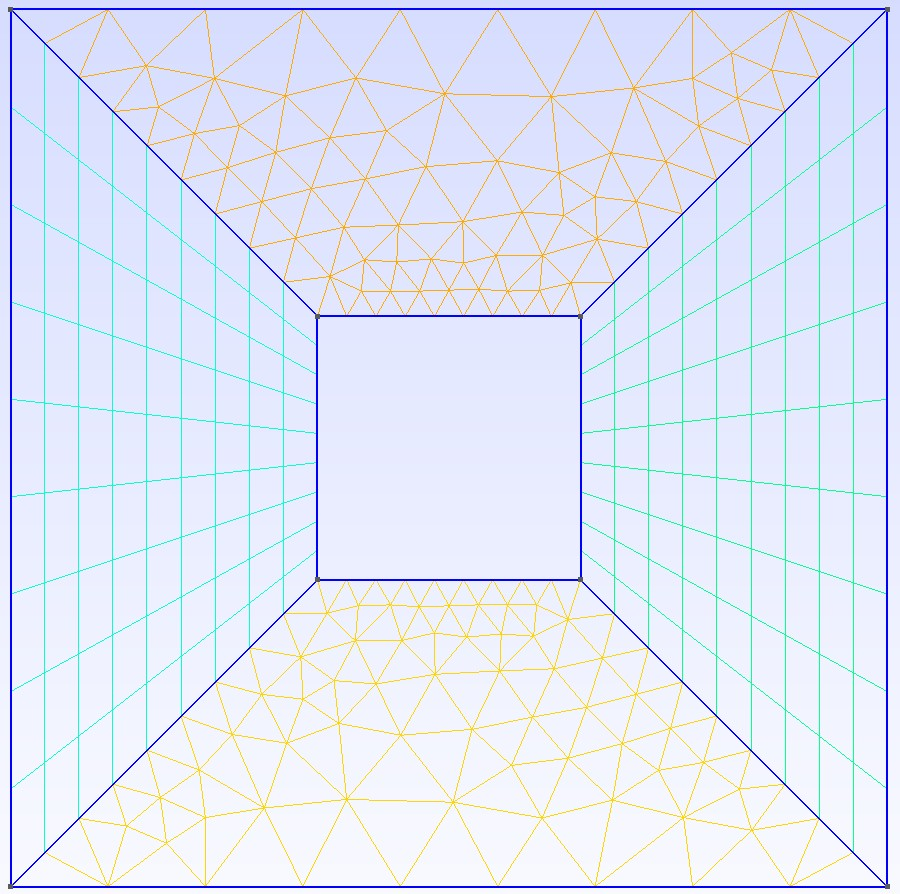
\includegraphics[width=0.4\linewidth, align=c]{onurk3.jpg} Figure 5 & {[[0.03082349],[0.00367857]]\newline[[0.00505206],[0.03057457]]} & {[[0.03074471],[0.00116142]]\newline[[0.00290107],[0.02801405]]} & {[[0.03321566],[0.00459645]]\newline[[0.0012708 ],[0.02808338]]}\\
        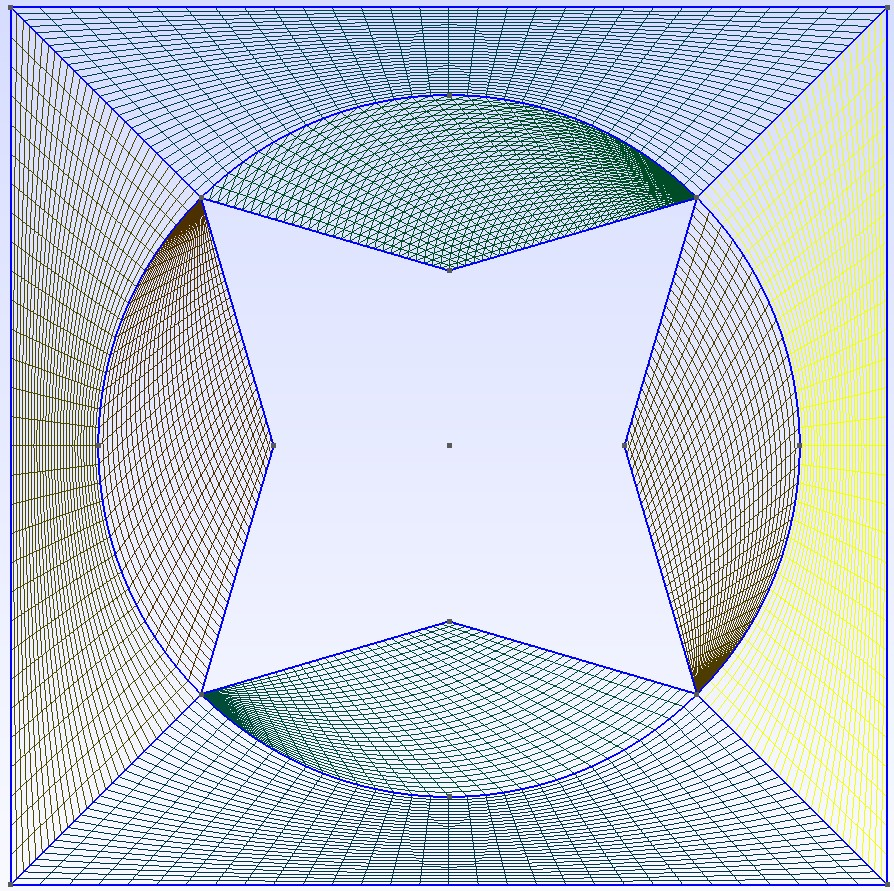
\includegraphics[width=0.4\linewidth, align=c]{alikmesh1.jpg} Figure 6 & {[[1.90565731],[1.89260198]]\newline[[0.09239694],[0.23073964]]} & {[[1.9165211 ],[1.89732045]]\newline[[0.07026629],[0.23439571]]} & {[[2.25920684],[2.2357312]]\newline[[0.09219926],[0.24661735]]}\\
        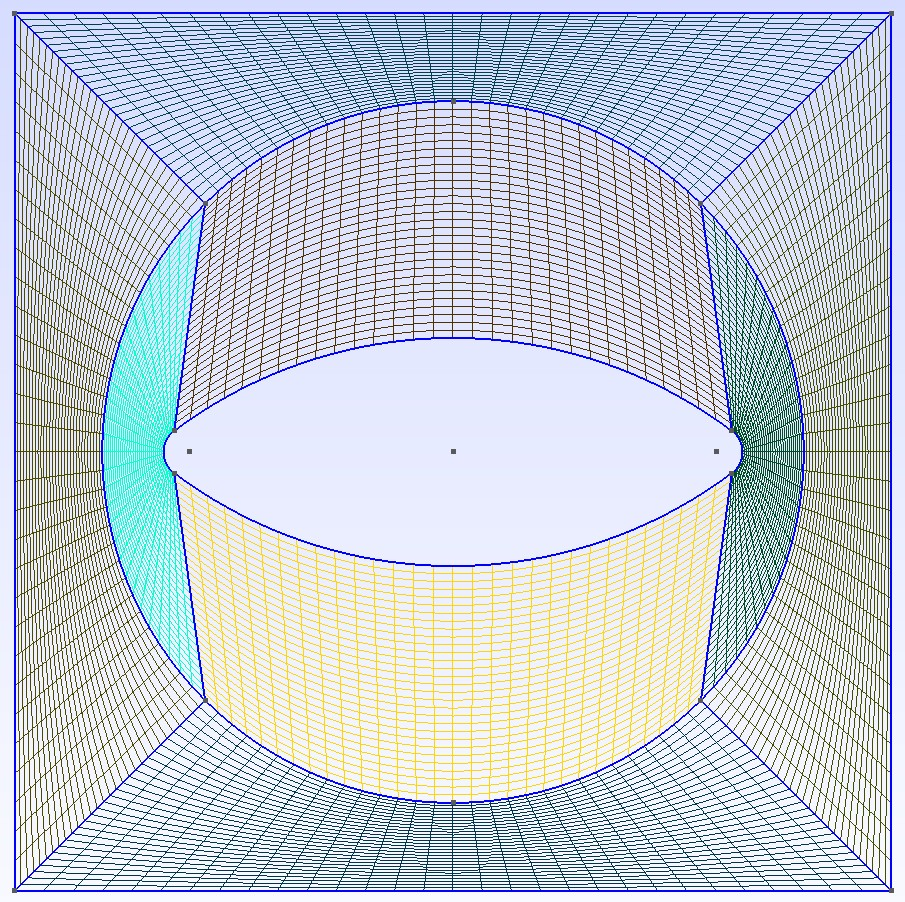
\includegraphics[width=0.4\linewidth, align=c]{alilk2.jpg} Figure 7 & [[1.88256696],[1.99961164]] & [[1.88497715],[1.99985048]] & [[2.22522845],[2.32094407]]\\
    \end{tblr}
    }
    \caption{Results for $q = \sqrt{x^2+y^2}$ Drichlet}
\end{table}
\begin{table}[H]
    \renewcommand\baselinestretch{1.1}\selectfont
    \centering
    \mbox{}\clap{
    \begin{tblr}
        []{
        rowsep = 0.5mm,
        colspec = {Q[c,m, 2cm]Q[c,m,4.7cm]Q[c,m,4.7cm]Q[c,m,4.7cm]},
        vlines, hlines}
        Mesh & $L_2$ Error Norm (GG) & $L_2$ Error Norm (LSQ) & $L_2$ Error Norm (wLSQ)  \\
       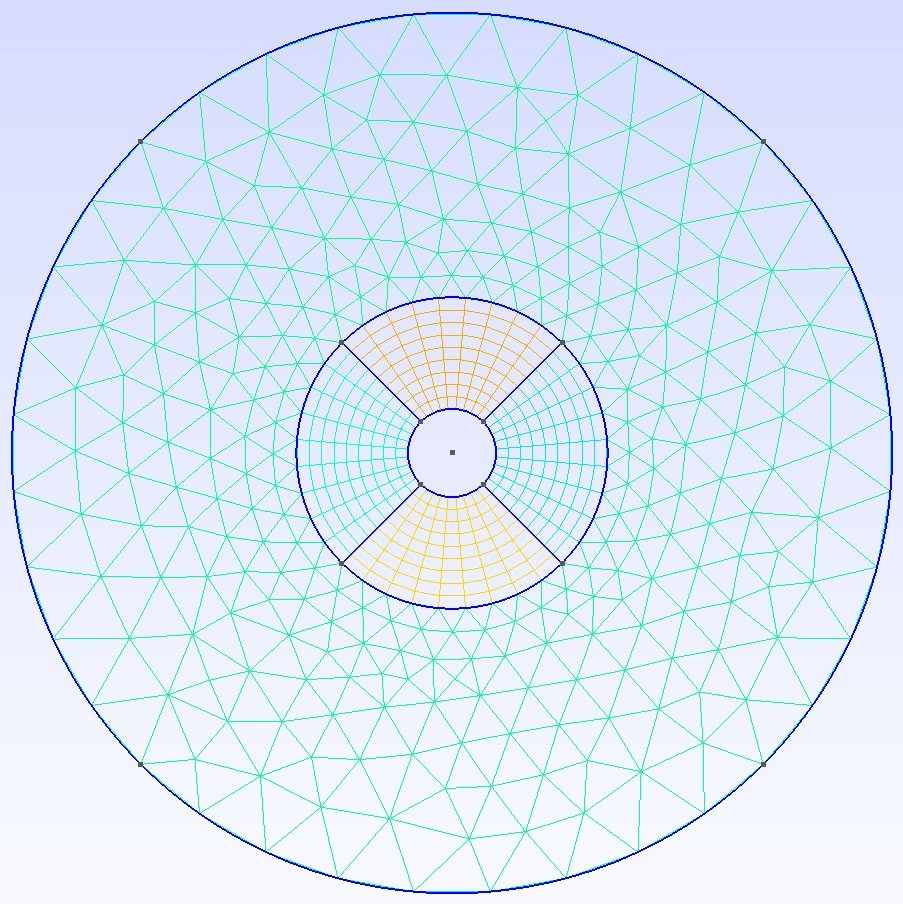
\includegraphics[width=0.4\linewidth, align=c]{grad.jpg} Figure 1 & {[[0.00131815],[0.0013341 ]]\newline[[0.105498],[0.10578135]]} & {[[0.0005871],[0.00058587]]\newline[[0.08760545],[0.08643159]]} &{[0.00036226],[0.00036214]]\newline[[0.08733679],[0.08672503]]}\\
       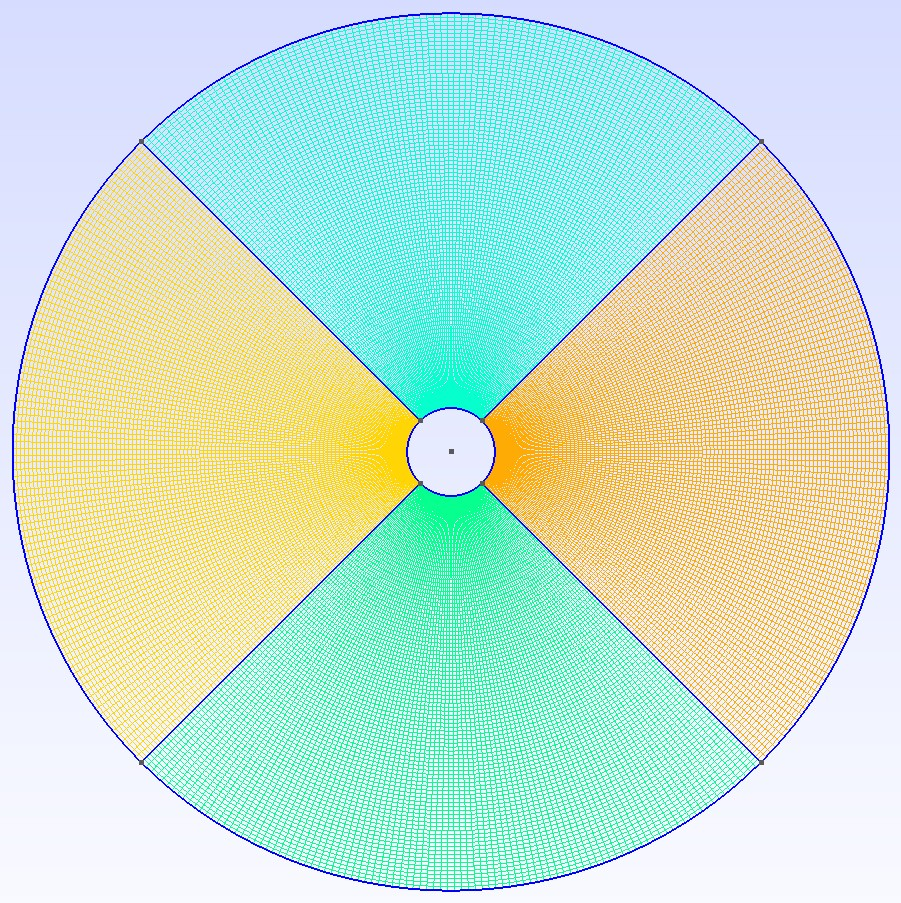
\includegraphics[width=0.4\linewidth, align=c]{grads.jpg} Figure 2 & [[0.00285672],[0.00285672]] & [[0.00284562],[0.00284562]] & [[0.00284453],[0.00284453]] \\
        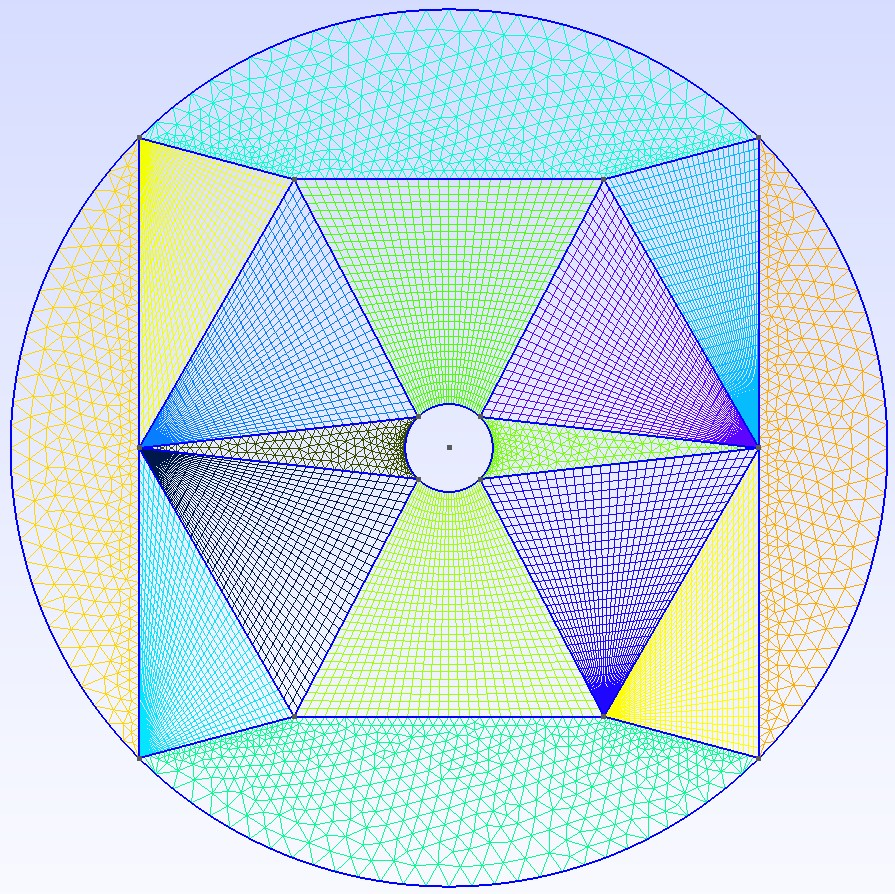
\includegraphics[width=0.4\linewidth, align=c]{onurk1.jpg} Figure 3 & {[[0.0039081 ],[0.00228413]]\newline[[0.02103257],[0.02094605]]} & {[[0.00018318],[0.00014021]]\newline[[0.01501804],[0.0149766]]} & {[[7.3987e-05],[1.1096e-04]]\newline[[0.01497567],[0.01486289]]} \\
        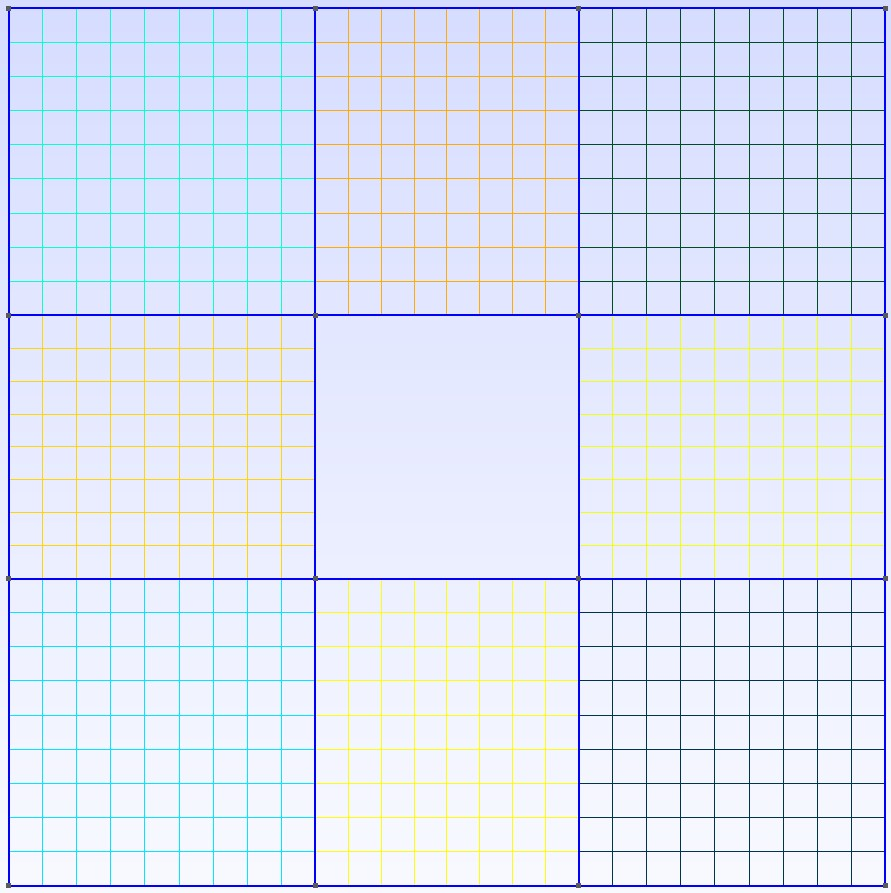
\includegraphics[width=0.4\linewidth, align=c]{onurk2.jpg} Figure 4 & [[0.0246458],[0.0246458]] & [[0.0246458],[0.0246458]] & [[0.02464564],[0.02464564]] \\
        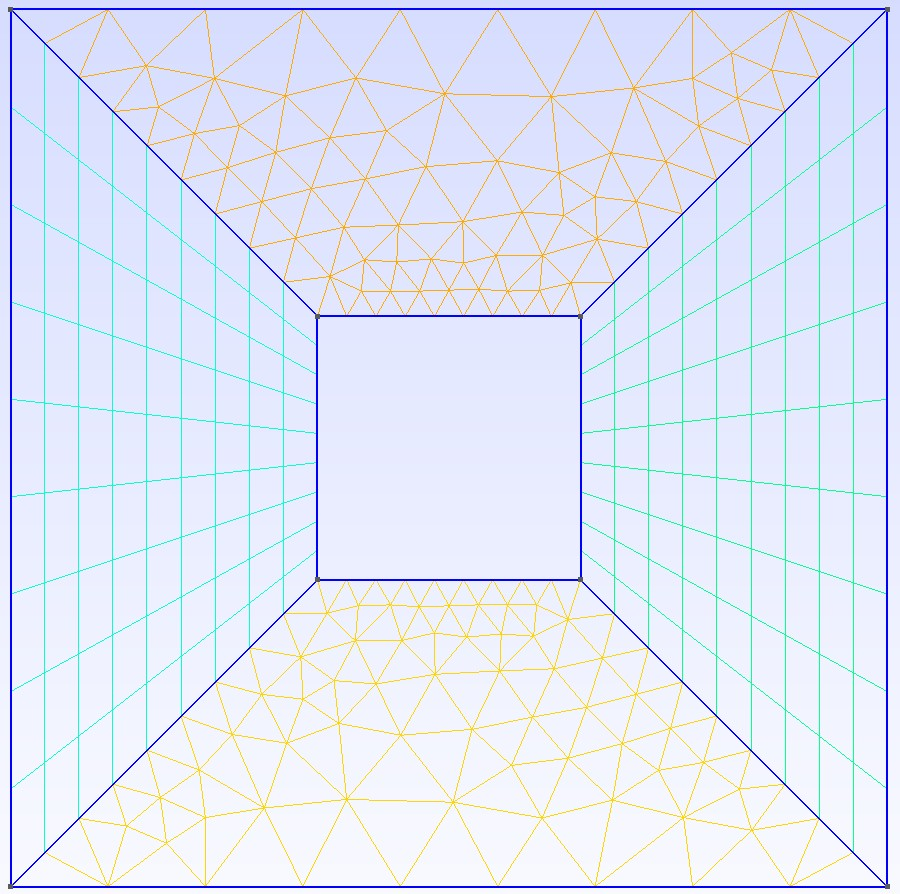
\includegraphics[width=0.4\linewidth, align=c]{onurk3.jpg} Figure 5 & {[[0.0382913],[0.00422454]]\newline[[0.00523682],[0.03859335]]} & {[[0.03802043],[0.00118542]]\newline[[0.0038781],[0.03555952]]} & {[[0.041346],[0.00584687]]\newline[[0.0016699],[0.03567757]]}\\
        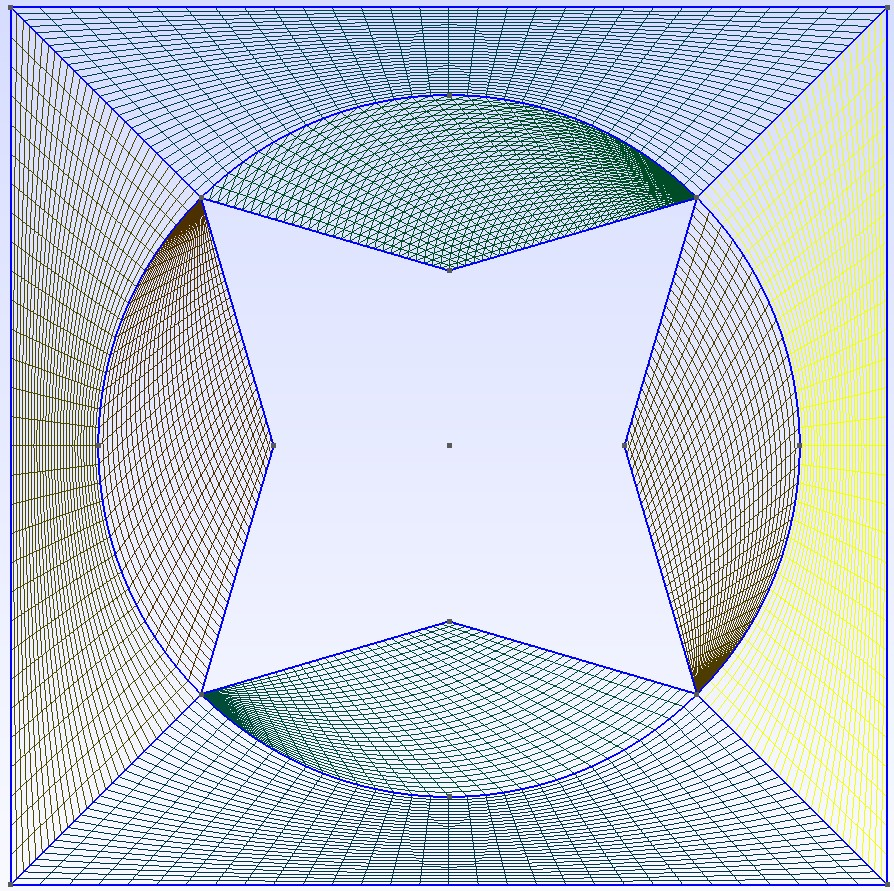
\includegraphics[width=0.4\linewidth, align=c]{alikmesh1.jpg} Figure 6 & {[[23.3627812],[23.3219324]]\newline[[0.56099016],[1.43135202]]} & {[[23.397633],[23.33718899]\newline[[0.42738759],[1.45156007]]} & {[[27.7407169],[27.6658563]]\newline[[0.56895783],[1.51328272]]} \\
        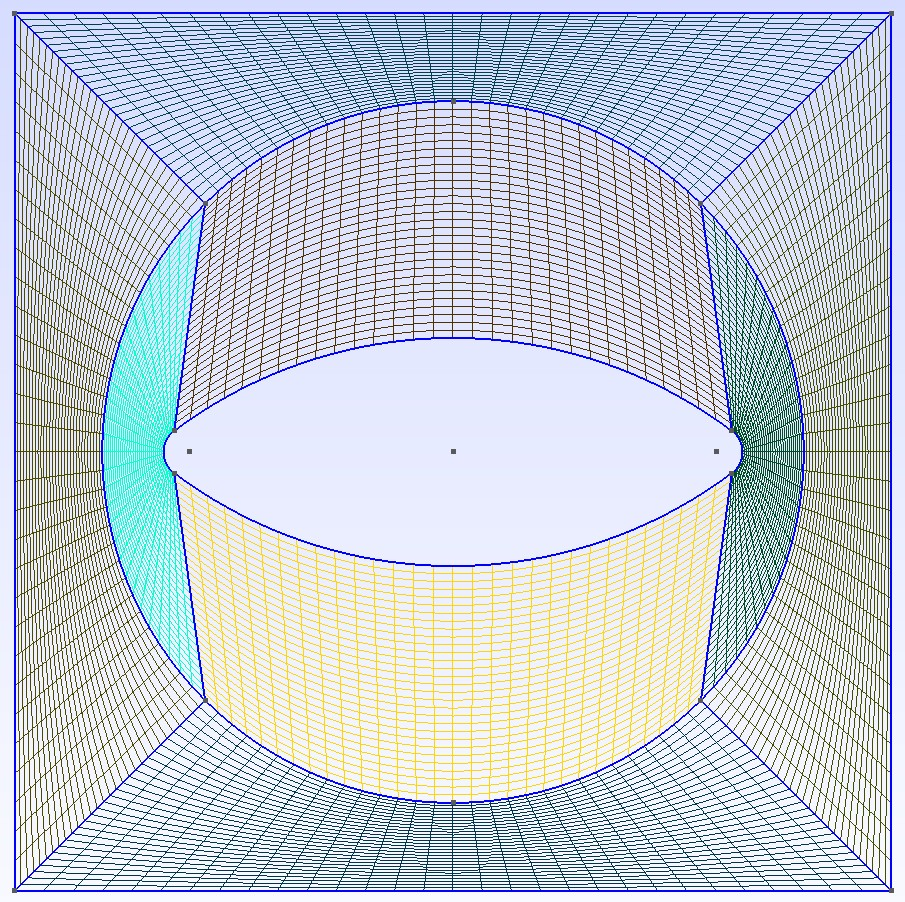
\includegraphics[width=0.4\linewidth, align=c]{alilk2.jpg} Figure 7 & [[23.2838976],[23.5061674]] & [[23.2898715],[23.5079755]] & [[27.6163662],[27.7956617]] \\
    \end{tblr}
    }
    \caption{Results for $q = x^2+y^2$ Drichlet}
\end{table}
\begin{table}[H]
    \renewcommand\baselinestretch{1.1}\selectfont
    \centering
    \mbox{}\clap{
    \begin{tblr}
        []{
        rowsep = 0.5mm,
        colspec = {Q[c,m, 2cm]Q[c,m,4.7cm]Q[c,m,4.7cm]Q[c,m,4.7cm]},
        vlines, hlines}
        Mesh & $L_2$ Error Norm (GG) & $L_2$ Error Norm (LSQ) & $L_2$ Error Norm (wLSQ)  \\
       \includegraphics[width=0.4\linewidth, align=c]{grad.jpg} Figure 1 & {[[90.9382921],[90.9382921]]\newline[[0.31523253],[0.3133322]]} & {[[103.356936],[103.356936]]\newline[[0.30020971],[0.29723711]]} & {[[102.965992],[102.965992]]\newline[[0.3014124 ],[0.30211584]]}\\
       \includegraphics[width=0.4\linewidth, align=c]{grads.jpg} Figure 2 & [[27.4535631],[27.4535631]] & [[28.7013832],[28.7013832]] & [[28.6996371],[28.6996371]] \\
        \includegraphics[width=0.4\linewidth, align=c]{onurk1.jpg} Figure 3 & {[[21.2471590],[45.1135171]]\newline[[45.1137279],[21.2476050]]} & {[[54.9763448],[38.0319801]]\newline[[45.0246162],[21.4202675]]} & {[[23.9674997],[47.4004365]]\newline[[43.8454258],[23.7877275]]} \\
        \includegraphics[width=0.4\linewidth, align=c]{onurk2.jpg} Figure 4 & [[0.00889283],[0.00889283]] & [[0.00889283],[0.00889283]] & [[0.00889283],[0.00889283]] \\
        \includegraphics[width=0.4\linewidth, align=c]{onurk3.jpg} Figure 5 & {[[0.01496869],[0.00158006]]\newline[[0.00176743],[0.01533238]]} & {[[0.01475973],[0.00053461]]\newline[[0.00163041],[0.01417951]]} & {[[0.01621377],[0.00236271]]\newline[[0.0007965 ],[0.01425679]]} \\
        \includegraphics[width=0.4\linewidth, align=c]{alikmesh1.jpg} Figure 6 & {[[1.99221924],[1.95506913]]\newline[[0.13669286],[0.40386797]]} & [[1.98197133],[1.9184128]]\newline[[0.10663218],[0.42126239]] & {[[2.22111504],[2.15260355]]\newline[[0.13141051],[0.42764634]]} \\
        \includegraphics[width=0.4\linewidth, align=c]{alilk2.jpg} Figure 7 & [[1.93051196],[1.98492893]] & [[1.87797907],[1.9347084]] & [[2.13312513],[2.16706029]] \\
    \end{tblr}
    }
    \caption{Results for $q = cos(x^2+y^2)$ Drichlet}
\end{table}
\begin{table}[H]
    \renewcommand\baselinestretch{1.1}\selectfont
    \centering
    \mbox{}\clap{
    \begin{tblr}
        []{
        rowsep = 0.5mm,
        colspec = {Q[c,m, 2cm]Q[c,m,4.7cm]Q[c,m,4.7cm]Q[c,m,4.7cm]},
        vlines, hlines}
        Mesh & $L_2$ Error Norm (GG) & $L_2$ Error Norm (LSQ) & $L_2$ Error Norm (w-LSQ)  \\
       \includegraphics[width=0.4\linewidth, align=c]{grad.jpg} Figure 1 & {[[5.8831e-11],[5.9212e-11]]\newline[[14614.5980],[14761.8929]]} & {[[5.2688e-11],[5.3015e-11]]\newline[[14341.5070],[14376.4434]]} & {[[4.6176e-11],[4.6361e-11]]\newline[[14476.3027],[14800.5200]]} \\
       \includegraphics[width=0.4\linewidth, align=c]{grads.jpg} Figure 2 & [[5295.0064],[5295.0064]] & [[5271.5776],[5271.5776]] & [[5272.1033],[5272.1033]] \\
       \includegraphics[width=0.4\linewidth, align=c]{onurk1.jpg} Figure 3 & {[[0.04038635],[0.00961823]]\newline[[10596.9569],[10652.1428]]} & {[[0.01646438],[0.00522647]]\newline[[10464.7119],[10495.0431]]} & {[[0.01743961],[0.00520740]]\newline[[10525.0680],[10410.7479]]} \\
       \includegraphics[width=0.4\linewidth, align=c]{onurk2.jpg} Figure 4 & [[1.7328e-11],[1.7328e-11]] & [[1.7328e-11],[1.7328e-11]] & [[1.7328e-11],[1.7328e-11]] \\
       \includegraphics[width=0.4\linewidth, align=c]{onurk3.jpg} Figure 5 & {[[3.1308e-11],[8.8478e-13]]\newline[[6.0220e-12],[5.4728e-11]]} & {[[2.6098e-11],[3.3802e-12]]\newline[[1.5130e-11],[4.9763e-11]]} & {[[3.7092e-11],[1.2308e-11]]\newline[[7.1365e-12],[4.7924e-11]]} \\
       \includegraphics[width=0.4\linewidth, align=c]{alikmesh1.jpg} Figure 6 & {[[2.5122e+22],[2.5122e+22]]\newline[[1.0466e+17],[2.8341e+17]]} & {[[2.4784e+22],[2.4784e+22]]\newline[[1.0106e+17],[2.2595e+17]]} & {[[3.1722e+22],[3.1722e+22]]\newline[[9.5219e+16],[3.8537e+17]]} \\
       \includegraphics[width=0.4\linewidth, align=c]{alilk2.jpg} Figure 7 & [[2.5122e+22],[2.5122e+22]] & [[2.4784e+22],[2.4784e+22]] & [[3.1722e+22],[3.1722e+22]] \\
    \end{tblr}
    }
    \caption{Results for $q = x^{32}+y^{32}$ Dirichlet}
\end{table}

\subsection{Comments}
\par In this section of the report various comments about the work done will be shared. Overall the results more or less follow the expected results. For instance, the most structural mesh, given in \hyperref[f4]{\textit{figure 4}}, has the smallest error norm out of all the meshes and test functions constructed by students. Furthermore; the highest error norms are achieved for all functions tested, which are the mesh structures shared at \hyperref[f6]{\textit{figure 6}} and \hyperref[f7]{\textit{figure 7}}.\\\par
Also as expected the $L_2$ error norm decreases as the number of elements increases. When the mesh depicted at \hyperref[here]{\textit{figure 2}} is adjusted for 1000 uniformly placed nodes, the $L_2$ error norm drops quite noticeably for both boundary conditions.\\\par
Comparison of Dirichlet and Neumann boundary conditions is next the comment will be shared. The result of this comparison is made by comparing the last two cases of Neumann to their Dirichlet counterparts. In short, this difference is caused by the errors introduced in the step of computing the boundary value for Dirichlet. For those who are interested, the reason behind this error has already been explained in \hyperref[s7.5]{\textit{Section 7.5}}. \\\par
The next comment is the comparison of trigonometric function cases for different element types. For the boundary type Neumann, $L_2$ norm and element type connection is highly dependent on geometry. Inspecting the shared results in \hyperref[T3]{\textit{Table 3}}, one can see that triangle elements have a lower $L_2$ norm compared to their quadrilateral counterparts. However, this changes towards the bottom of the table. for distorted geometries, quadrilateral meshes work better. When it comes to Dirichlet boundary conditions no matter what the geometry is, triangle elements resulted in a lower $L_2$ norm compared to quadrilateral ones. This trend continues for higher-order functions.\\\par
Another comment is the comparison of the gradient calculating method on the same geometry. Catching a generic trend is not possible for the test cases presented. In theory, it is expected to have the $L_2$ norm decrease as the method shifts from Green-Gauss to weighted Least Squares. However, data from \hyperref[T1]{\textit{Table 1}}, follows the theory near perfect for the first three cases, for the last four cases $L_2$ first decreases then increases. This continues for the second table as well. However, from the third table to the last table for the Neumann condition, the $L_2$ norm follows the theory. Regarding the Dirichlet condition, the "first increase and then decrease" trend is presented for all tables indifferent to the input equation type. Yet for the first case, the trend follows a decreasing pattern, for the cases from two to seven it follows the trend "first decrease then increase". So it is not wrong to say that as geometry gets more complex Least Squares method without a weighting factor causes less error, yet this result may not be one hundred percent correct since even though the norms are lower in Green Gauss compared to Least Squares, they are still pretty high to run a healthy CFD simulation. \\\par
Adding one more comment about the $L_2$ norm can be that the norm also increases as the functions' nonlinearity increases. One can see this trend by comparing the norm values for the same geometry on different tables.\\\par
For test case six and case seven outer dimensions and the circle at the middle are the same, further in both the regions where lies between the outer boundary and the middle circle are meshed via quadrilateral. Due to these similarities, their $L_2$ error norm for quad elements is pretty much the same. This trend remains unchanged for both Dirichlet and Neumann boundary conditions.\\\par
The last comment is, that in structured mesh, test case four, $L_2$ error norm, changes slightly in the case of Neumann-type boundary conditions, but for Dirichlet-type boundary conditions it will yield the same values regardless of what the boundary functions are.

\newpage
\section{References}
\begin{itemize}
    \item Ali Karakuş Github Repo for \mefvm - \textcolor{blue}{\href{https://github.com/AliKarakus/me485-HWs/tree/HW1}{link}}
    \item Ali Karakuş Lecture Notes for ME485 - \textcolor{blue}{\href{https://odtuclass2024f.metu.edu.tr/course/view.php?id=2835}{link}}
\end{itemize}
\end{document}